\documentclass[
	12pt,
  twoside,
  stile=classica,
  oldstyle,
  tipotesi=magistrale,
  numerazioneromana,
  cucitura=7mm
]{toptesi}

\usepackage[utf8]{inputenc}
\usepackage[T1]{fontenc}
\usepackage{lmodern}
\usepackage[english]{babel}

\usepackage{hyperref}

\usepackage[backend=biber]{biblatex}

\usepackage{lipsum} 
\usepackage{amsmath, amssymb}
\usepackage{appendix}
\usepackage{longtable}
\usepackage{lscape}
\usepackage{adjustbox}
\usepackage{float}
\usepackage{accsupp}
\usepackage{blindtext}
\usepackage{setspace}
\usepackage{parskip}
\usepackage{array}
\usepackage{titlesec}
\usepackage{geometry} 
\usepackage{dcolumn}

\usepackage[toc, abbreviations, nonumberlist]{glossaries-extra}

\usepackage{afterpage}
\usepackage{listings}
\usepackage{xcolor}
\usepackage{tabularx}
\usepackage{makecell}
\setabbreviationstyle{long-short-desc}

\hypersetup{
    pdfpagemode={UseOutlines},
    bookmarksopen,
    pdfstartview={FitH},
    colorlinks,
    linkcolor={blue},
    citecolor={red},
    urlcolor={black}
}

\titleformat{\subsubsection}[hang]{\normalfont\normalsize\bfseries}{\thesubsubsection}{1em}{}
\titlespacing*{\subsubsection}{0pt}{\baselineskip}{\baselineskip}
\titleformat{\paragraph}[hang]{\normalfont\normalsize\bfseries}{\theparagraph}{1em}{}
\titlespacing*{\paragraph}{0pt}{\baselineskip}{\baselineskip} 

\newcommand\fillin[1][4cm]{\makebox[#1]{\dotfill}} 

\newcommand\blankpage{
  \null
  \thispagestyle{empty}
  \addtocounter{page}{-1}
  \newpage
}

\renewcommand\theadfont{\bfseries}

\definecolor{codegray}{rgb}{0.5,0.5,0.5}
\definecolor{lightgray}{rgb}{.9,.9,.9}
\definecolor{darkgray}{rgb}{.4,.4,.4}
\definecolor{purple}{rgb}{0.65, 0.12, 0.82}
\definecolor{yellow}{rgb}{1.0, 0.8, 0.2}
\definecolor{lightblue}{rgb}{0.53, 0.81, 0.98}
\definecolor{darkblue}{rgb}{0.0, 0.0, 0.55}
\definecolor{green}{rgb}{0.0, 0.5, 0.0}

\lstdefinelanguage{JavaScript}{
  backgroundcolor=\color{lightgray},
  keywords={Promise, Error, Buffer, Resolver, EthrDID, PRIV_KEY, OWN_ADDRESS, typeof, catch, function, return, null, catch, switch, var, if, in, while, do, else, case, break, try, await},
  keywordstyle=\color{purple}\bfseries,
  identifierstyle=\color{lightblue},
  sensitive=false,
  comment=[l]{//},
  morecomment=[s]{/*}{*/},
  commentstyle=\color{green},
  stringstyle=\color{green},
  morestring=[b]',
  morestring=[b]",
  basicstyle=\small\ttfamily,
  showstringspaces=false, 
  numberstyle=\tiny\color{codegray},
  breakatwhitespace=false,         
  breaklines=true,                 
  captionpos=b,                    
  keepspaces=true,                                    
  numbersep=5pt,                  
  showspaces=false,       
  showtabs=false,                  
  tabsize=2,
  frame=single,
  numbers=left,
  morekeywords=[2]{reload, setErrorMessage, clearError, wait, registerUser, Contract, isRegistered, signupDataCellar, timeoutPromise, race, getSigner, BrowserProvider, deployed, deploy, log, require, removeListener, updateWalletAndAccounts, getProvider, setHasProvider, detectEthereumProvider, on, length, setWallet, useCallback, request, updateWallet, parseInt, getResolver, verifyCredential, _updateWallet, getContract, verifyVc, navigate, setAuthState, handleLoggedIn, useEffect, find, split, UnauthorizedException, generatePayload, toLowerCase, recoverPersonalSignature, bufferToHex, generateJwtToken, signAsync, createVerifiableCredentialJwt, generateVcPayload, generateVerifiableCredential, },
  keywordstyle=[2]\color{orange}\bfseries,
  morekeywords=[3]{async, true, false, class, const, new, export, boolean, throw, implements, import, this},
  keywordstyle=[3]\color{darkblue}\bfseries 
}

\lstdefinelanguage{Solidity}{
  backgroundcolor=\color{lightgray},
  keywords={pragma, contract, function, return, constructor, public, private, external, internal, payable, view, pure, event, emit},
  keywordstyle=\color{blue}\bfseries,
  ndkeywords={address, uint, string, bool, mapping, struct, require, keccak256},
  ndkeywordstyle=\color{darkgray}\bfseries,
  identifierstyle=\color{black},
  sensitive=false,
  comment=[l]{//},
  morecomment=[s]{/*}{*/},
  commentstyle=\color{purple},
  stringstyle=\color{red},
  morestring=[b]',
  morestring=[b]",
  basicstyle=\small\ttfamily,
  showstringspaces=false, 
  numberstyle=\tiny\color{codegray},
  breakatwhitespace=false,         
  breaklines=true,                 
  captionpos=b,                    
  keepspaces=true,                 
  numbers=left,                    
  numbersep=5pt,                  
  showspaces=false,       
  showtabs=false,                  
  tabsize=2,
  frame=single
}

\lstdefinelanguage{JWT}{
  keywords={alg, typ, iss, sub, aud, exp, nbf, iat, jti},
  keywordstyle=\color{blue}\bfseries,
  ndkeywords={},
  ndkeywordstyle=\color{darkgray}\bfseries,
  identifierstyle=\color{black},
  sensitive=false,
  comment=[l]{//},
  morecomment=[s]{/*}{*/},
  commentstyle=\color{purple},
  stringstyle=\color{red},
  morestring=[b]',
  morestring=[b]",
  basicstyle=\small\ttfamily,
  showstringspaces=false, 
  numberstyle=\tiny\color{codegray},
  breakatwhitespace=false,         
  breaklines=true,                 
  captionpos=b,                    
  keepspaces=true,                 
  numbers=left,                    
  numbersep=5pt,                  
  showspaces=false,       
  showtabs=false,                  
  tabsize=2,
  frame=single
}


\addbibresource{references.bib}

\newacronym{ssi}{SSI}{Self Sovereign Identity}
\newacronym{dapp}{DApp}{decentralized application}
\newacronym{dlt}{DLT}{Distributed Ledger Technology}
\newacronym{mempool}{MemPool}{Memory Pool}
\newacronym{pow}{PoW}{Proof of Work}
\newacronym{pos}{PoS}{Proof of Stake}
\newacronym{sha2}{SHA-2}{Secure Hash Algorithm 2}
\newacronym{utxo}{UTXO}{Unspent Transaction Output}
\newacronym{pki}{PKI}{Public Key Infrastructure}
\newacronym{pin}{PIN}{Personal Identification Number}
\newacronym{arpanet}{ARPANET}{Advanced Research Projects Agency Network}
\newacronym{ip}{IP}{Internet Protocol}
\newacronym{idp}{IDP}{Identity Provider}
\newacronym{did}{DID}{Decentralized Identifier}
\newacronym{vc}{VC}{Verifiable Credential}
\newacronym{idm}{IDM}{Identity Management}
\newacronym{sso}{SSO}{Single Sign-On}
\newacronym{pgp}{PGP}{Pretty Good Privacy}
\newacronym{w3c}{W3C}{World Wide Web Consortium}
\newacronym{ddo}{DDO}{DID Document}
\newacronym{uri}{URI}{Uniform Resource Identifier}
\newacronym{vp}{VP}{Verifiable Presentation}
\newacronym{zkp}{ZKP}{Zero-Knowledge Proof}
\newacronym{dht}{DHT}{Distributed Hash Table}
\newacronym{ipfs}{IPFS}{Interplanetary File System}
\newacronym{tee}{TEE}{Trusted Execution Environment}
\newacronym{eddsa}{EdDSA}{Edwards-curve Digital Signature Algorithm}
\newacronym{ecdsa}{ECDSA}{Elliptic Curve Digital Signature Algorithm}
\newacronym{ddos}{DDoS}{Distributed Denial of Service}
\newacronym{abi}{ABI}{Application Binary Interface}
\newacronym{api}{API}{Application Programming Interface}
\newacronym{jwt}{JWT}{JSON Web Token}
\newacronym{sdk}{SDK}{Software Development Kit}
\newacronym{cli}{CLI}{Command Line Interface}
\newacronym{idms}{IDMS}{Identity Management System}
\newacronym{nonce}{Nonce}{Number used once}
\newacronym{gui}{GUI}{Graphical User Interface}
\newacronym{eu}{EU}{European Union}
\newacronym{https}{HTTPS}{Hypertext Transfer Protocol Secure}
\newacronym{ssl}{SSL}{Secure Sockets Layer}

\makeglossaries

%%%%%%%%%%%%%%%%%%%%%%%%%%%%%%%%%%%%%%%%%%%%%%%%
%%%%%%%%%%%%%%%%%%%%%%%%%%%%%%%%%%%%%%%%%%%%%%%%

\begin{document}
\errorcontextlines=9
\english
\pagestyle{empty}

\begin{titlepage}

  \newgeometry{left=1cm,right=1cm,top=3cm,bottom=3cm}

  \begin{center}

    {\huge POLITECNICO DI TORINO}\\[1cm]

    
\includegraphics[width=0.3\textwidth]{./Images/logo_polito_2021.jpg}

    \textbf{\large Master’s Degree in Computer Engineering\\Cybersecurity Focus}\\[3cm]

    %{\Large Tesi di Laurea}\\[1cm]

    \textbf{\huge Decentralized Identity Management: Building and Integrating a Self-Sovereign Identity Framework }\\[2cm]
    \vspace{3.5cm}

    \begin{minipage}{0.85\textwidth}

      \begin{flushleft}\large
        \textbf{Supervisor} \hfill \textbf{Candidate}\\
        Prof. Danilo Bazzanella\hfill Luca Rota\\
      \end{flushleft}

      \begin{flushleft}\large
        \textbf{Company Supervisors} \\
        Dr. Alfredo Favenza\\
        Dr. Silvio Meneguzzo\\
      \end{flushleft}

    \end{minipage}

    \vfill

    Accademic Year 2023/2024
  \end{center}

  \restoregeometry

\end{titlepage} 

\afterpage{\blankpage}

%%%%%%%%%%%%%%%%%%%%%%%%%%%%%%%%%%%%%%%%%%%%%%%%
%%%%%%%%%%%%%%%%%%%%%%%%%%%%%%%%%%%%%%%%%%%%%%%%

\sommario
In the revolution of technology that is known in this era, identity has transitioned from its original forms to the digital area. Such change in paradigm requires the 
re-evaluation of identity management issues and in this context the Self-Sovereign Identity (SSI) is the most relevant concept.

This thesis, conducted at Links Foundation, investigates the evolving ecosystem of Self-Sovereign Identity (SSI) in the context of decentralized identity management. 
Employing the blockchain technology and MetaMask, a SSI standalone framework is developed and later integrated into the Data Cellar project of Links Foundation, thus showing practical usability.
By digging into thoroughly cryptographic and cybersecurity aspects, the research ends in a decentralized application (DApp),combining a frontend 
elegance (React, JS) and a robust backend (NestJs) for secure and user-centric authentication.

Decentralized identity is an area of ongoing discussion, and this work falls in line with Links Foundation direction of digital innovation.

\ringraziamenti

Before proceeding with the discussion, I would like to dedicate a few lines to all those who have been close to me in this path of personal and professional growth.

First and foremost, I would like to thank my advisor Bazzanella and my co-advisors Meneguzzo and Favenza, who were always ready to give me the right guidance, at every stage of the realization of the thesis. 

I am grateful to the Links Foundation, for giving me the opportunity to do my thesis work in a dynamic place and gain an experience that will be invaluable for my future. 

I thank infinitely my mother, father, sister, and the rest of my family; without their constant support and teachings, I would not be who I am today. Without you, this would not have been possible.

Heartfelt thanks also go to my girlfriend, Beatrice, for her patience, understanding and unwavering sustenance during this journey. Her trust in me has been a constant source of motivation.

To my old friends in Liguria and my new friends in Turin; thank you for loving me for who I am, for always being by my side, and for all the carefree times we spent together.

Finally, I dedicate this thesis to myself and to my sacrifices and tenacity that have allowed me to get this far.

\afterpage{\blankpage}

%%%%%%%%%%%%%%%%%%%%%%%%%%%%%%%%%%%%%%%%%%%%%%%%
%%%%%%%%%%%%%%%%%%%%%%%%%%%%%%%%%%%%%%%%%%%%%%%%

\cleardoublepage
\pagestyle{plain}

\tableofcontents

\listoftables

\listoffigures

\addcontentsline{toc}{chapter}{Listings}
\lstlistoflistings

\printunsrtglossary[title=Acronyms,type=\glsxtrabbrvtype]

\cleardoublepage
\thispagestyle{empty}
\mbox{}

\setcounter{page}{1}
\pagenumbering{arabic}

%%%%%%%%%%%%%%%%%%%%%%%%%%%%%%%%%%%%%%%%%%%%%%%%
%%%%%%%%%%%%%%%%%%%%%%%%%%%%%%%%%%%%%%%%%%%%%%%%

\mainmatter

\chapter{Introduction} \label{ch:introduction}

In a world of constantly advancing technology, the concept of identity has experienced significant transformation. Managing identity becomes a critical issue in this
time when our lives are becoming bound by digital platforms, services and, networks. Centralized identity systems, being popular, are however, encumbered by 
issues like the lack of user control and data breaches. As an answer to the above mentioned challenges, the idea of \acrfull{ssi} has been gaining more attention. \gls{ssi} 
adopts a decentralized and user-centric approach to identity management that enables individuals to assert and manage control over their identity data effectively. 
Through blockchain technology, \gls{ssi} enables a secure and trust-based architecture of identity verification, where intermediaries are not required and identity is 
protected from theft. The present research centers on the terrain of digital identity, especially concentrating on the standards and implementations of \gls{ssi}.

\section{Objectives} 

This thesis delves into the ever-evolving ecosystem of Links Foundation to thoroughly explore the concept of \gls{ssi}. Our ambitious objectives 
are to develop an autonomous \gls{ssi} framework for managing decentralized identities by using MetaMask and the Ethereum blockchain. Furthermore, we strive to 
seamlessly incorporate this cutting-edge framework into the advanced Data Cellar project at Links Foundation.

Link Foundation is an innovative organization that facilitates digital transformation via applied research, innovation, and technology transfer projects \cite{linksfoundation}.
Founded by the collaboration between the Compagnia di San Paolo and the Politecnico di Torino, the Links foundation is the central part of different technical and scientific 
disciplines, developing projects raging from Artificial Intelligence to Cybersecurity.

This exploration takes us into the intricacies of technology tracing the origins of identity from its non digital beginnings to its current form. By studying the foundations
of \gls{ssi} we gain insights, into the security and privacy measures in place as well as addressing the prevalent cybersecurity challenges within the \gls{ssi} domain.

With a focus on practicality this research culminates in developing a \gls{ssi} framework that incorporates groundbreaking elements like MetaMask and a customized Ethereum smart 
contract. This framework has the potential to revolutionize identity management, as evidenced by its integration into Data Cellar.

As we reach the end of this journey, we celebrate achieving an accomplishment, creating a \acrfull{dapp}. This achievement not showcases an user friendly interface 
built with React and JS for frontend development and NestJs for backend development but also seamlessly integrates our \gls{ssi} framework. This milestone not overcomes standing 
obstacles but also paves the way, for a future where individuals have greater control over their digital identities.

\section{Outline}

After a brief introduction and description of the goals of the thesis presented in Chapter \hyperref[ch:introduction]{[1]}, the remainder of the paper is structured as follows:

\begin{itemize}
  \item \textbf{Chapter \hyperref[ch:blockchain]{[2]}}: This chapter, therefore, is all about the background of the \gls{ssi} model used in 
  this study, which is blockchain technology. It starts with the definition and roles of blockchain, passes to the analysis of different types of blockchains, and ends 
  with a comparative review of two famous existing blockchains, namely Bitcoin and Ethereum.
  \item \textbf{Chapter \hyperref[ch:identity]{[3]}}: In this relatively concise chapter, an introduction to identity is provided, encompassing its evolutionary history 
  from the pre-digital era to a comparison of the three primary paradigms utilized for digital identity management: centralized , federated and user-centric.
  \item \textbf{Chapter \hyperref[ch:ssi]{[4]}}: This chapter focuses on the main theme of the thesis, namely the \gls{ssi} model. It evaluates the state-of-the-art of this 
  model of leading by starting from its historical context, then defining its main principles and presenting its advantages. Subsequently, the three main components of a 
  \gls{ssi} system, consist of \gls{did}, \gls{vc}, and Verifiable Data Registry, will be discussed 
  followed by an architecture analysis with a main focus on the "Trust Triangle" relation between the three principal entity: holder, verifier, and issuer.
  \item \textbf{Chapter \hyperref[ch:security]{[5]}}: According to the previous chapter's theme, this paragraph goes further to provide an in-depth study of the other 
  strong cryptographic and cybersecurity aspects of the \gls{ssi} model. Firstly, it highlights the working of VC proofs and then analyzes the attack vectors and their 
  vulnerabilities to which this model is prone.
  \item \textbf{Chapter \hyperref[ch:framework]{[6]}}: This chapter ends with the theoretical part and starts the practical discussion applied during the thesis period. 
  Overall, it explains the whole procedure of building an independent framework to handle the digital identities of individuals in a decentralized way under the \gls{ssi} model. 
  It demonstrates the instruments used for its implementation, the limitations encountered, and the final result.
  \item \textbf{Chapter \hyperref[ch:integration]{[7]}}: In this subsequent chapter, the integration of the previously mentioned framework into a practical project will be 
  presented to show its practical significance. It provides a brief background of the project and then proceeds to a comprehensive analysis before and after integration.
  \item \textbf{Chapter \hyperref[ch:conclusions]{[8]}}: This final chapter summarize the conclusions drawn from the research.It begins with a succinct summary outlining 
  the primary thesis topic and the executed practical endeavors, followed by an exposition of potential future work avenues necessitated by encountered limitations.
\end{itemize}

\chapter{The Blockchain Technology} \label{ch:Blockchain}

In the current landscape, blockchain technology has attracted increasing global interest due to its promising applications and potential transformative impacts on various 
sectors. Founded in 2008 by Satoshi Nakamoto as the mainstay of the Bitcoin system \cite{9752154}, blockchain has evolved from a simple ledger of financial transactions 
to a fundamental technology that revolutionizes the way information is recorded, shared and managed within decentralized networks.

\section{What is the Blockchain}

The blockchain is a core technology that drives many decentralized systems offering transparency, trust and safety without having to have a central authority. It is 
basically a distributed ledger that operates through the peer-to-peer \cite{9596538}, \cite{ibm_blockchain}. This section talks of the key components and architecture in 
blockchain, revealing its fundamental features and operating principles.

\subsection{Core Elements of Blockchain}

The blockchain comprises several key elements essential to its functionality:

\begin{itemize}
  \item \textbf{Blocks}: A block is a basic unit comprising of transactional data. Every block is securely connected to the previous one; this connection creates a chain 
  of blocks. The transactions within a block are cryptographically secured; hence, immutability and integrity \cite{9596538}, \cite{ibm_blockchain}.
  \item \textbf{Transactions}: Transactions are diverse interactions in the blockchain network. These interactions are not limited to the financial transfers only; any 
  piece of valuable information can be considered as a transaction and diffused within the network \cite{9752154}, \cite{9036241}.
  \item \textbf{Decentralization}: Unlike centralized systems that depend on a single controlling authority, the blockchain is decentralized. It includes a web of 
  interdependent nodes, each replicating the distributed registry. Resilience, transparency and no single points of failure are guaranteed by decentralization \cite{9596538}, \cite{9752154}.
  \item \textbf{Consensus Mechanism}:  For verification and agreement of the state of a ledger, blockchain uses consensus mechanisms. The most common mechanism, \gls{pow}, 
  requires miners to solve the complicated cryptographic puzzles in order to add new blocks on the chain. Consensus mechanisms ensure consensus among network participants 
  to prevent attacks by malicious actors \cite{9596538}, \cite{9752154}.
\end{itemize}

\subsection{Blockchain Architecture}

The structure of the system is carefully crafted to uphold its principles of decentralization, immutability and transparency;

\begin{itemize}
  \item \textbf{\gls{dlt}}: At the core of blockchain lies DLT, where all participants, in the network have access to a ledger of transactions. 
  This shared ledger eliminates redundancy. Ensures that everyone has a trusted source of information across the network \cite{ibm_blockchain}, \cite{9752154}.
  \item \textbf{Immutable Records}: One key feature of blockchain is its records immutability. Once a transaction is recorded on the ledger it cannot be. Tampered with. 
  Any attempt to change a transaction requires adding an one preserving the integrity of data \cite{ibm_blockchain}.
  \item \textbf{Smart Contracts}: Smart contracts are self executing contracts with predefined rules embedded within the blockchain. These contracts. Enforce agreements 
  between parties speeding up transaction processing and reducing reliance on intermediaries \cite{ibm_blockchain}, \cite{9036241}.
  \item \textbf{Security Measures}:  Cryptography plays a role in ensuring security by protecting transactions from tampering and fraud. Private key pairs authenticate. 
  Enable secure digital identity management. Additionally cryptographic hashing guarantees data integrity and confidentiality \cite{9596538}, \cite{9036241}.
  \item \textbf{Peer-to-Peer Network}: The blockchain functions using a network architecture where participants can directly communicate and interact. This decentralized 
  structure promotes trust and resilience since transactions are verified and validated through consensus, among distributed nodes \cite{9752154}, \cite{9036241}.
\end{itemize}

\section{How the Blockchain works}

The function of a blockchain system encompasses a complex chain of procedures that safeguard the  integrity, transparency, and security of transactions. In this section, 
we delve into the fundamental mechanisms of blockchain.

\subsection{Transaction process}

\paragraph{Recording transactions}

\begin{enumerate}
    \item \textbf{Starting a Transaction:} In a network, users initiate transactions through their wallets. Each wallet has a pair of keys. A key, for starting transactions 
    and a private key for authentication \cite{9596538}.
    \item \textbf{Creating Blocks:} As transactions take place they are grouped together into blocks of data. These blocks act as containers for recording details like 
    asset movement participants involved and timestamps \cite{ibm_blockchain}.
    \item \textbf{Hashing:} Every block contains information and refers to the hash of the previous block. Secure hash functions like SHA 256 play a role in ensuring the 
    integrity and immutability of transactions. Hashing allows each block to have a fingerprint making identification and verification simple \cite{ibm_blockchain} ,\cite{9036241}.
\end{enumerate}

\paragraph{Consensus Mechanism}

\begin{enumerate}
    \setcounter{enumi}{3}
    \item \textbf{Verification Process:} When a transaction is initiated the information is sent to a network of distributed peer, to peer nodes. These nodes work together 
    to confirm the validity of transactions using consensus mechanisms \cite{9036241}, \cite{geeksforgeeks}.
    \item \textbf{Formation of New Blocks:} Valid transactions are added to a \gls{mempool} where they wait to be included in a block. Miners, who are responsible 
    for creating blocks solve cryptographic puzzles in order to mine blocks. This process, known as \gls{pow} requires resources and time \cite{9596538}, \cite{geeksforgeeks}.
    \item \textbf{Consensus Algorithm:} In order to add a block to the blockchain nodes must agree on its validity through consensus algorithms. The miner who successfully 
    creates a block is rewarded. Consensus algorithms ensure that all nodes are synchronized and in agreement, about the state of the blockchain \cite{geeksforgeeks}.
    \item \textbf{Blockchain Integrity:} The interconnected nature of blocks ensures the immutability and integrity of the blockchain. Each block references the hash value 
    of its predecessor making it practically impossible to tamper with transactions without altering blocks \cite{9596538} ,\cite{9036241}.
\end{enumerate}

\subsection{Blockchain Benefits}

Due to the execution process described above and its architecture, blockchain is able to offer many benefits in different areas:

\begin{itemize}
  \item \textbf{Greater Trust:} Blockchain helps establish trust across the network through utilizing the decentralized ledger, making sure that data is consistent and 
  timely plus, it doesn’t require intermediaries \cite{9596538}. 
  \item \textbf{Enhanced Security:} Blockchain's security features are designed to thwart tampering as well as cybercrime. The blockchain structures transactions as 
  read-only data which is difficult to change and ensures that the data is protected even when it is in transit. Moreover, cryptography is used as a mechanism of 
  verification and the cryptographic infrastructure is used to store and transmit secrets \cite{ibm_blockchain}.
  \item \textbf{Time Savings:} The utilization of blockchain technology decreases greatly the processing time for transactions since they get completed within a quarter of 
  an hour due to the removal of the centralized authority that confirms \cite{ibm_blockchain}.
  \item \textbf{Cost Savings:} The blockchain adjusts transaction procedure and lowers operational costs by the removal of intermediaries, as tasks are automated and there 
  is lower duplication of activities through the usage of shared ledger \cite{9596538}, \cite{9036241}.
  \item \textbf{Efficiency Improvements:} The distributed architecture of blockchain increases system resilience, decreases processing costs, and removes the need for 
  centralized network control by distributing network operations thinly, facilitating faster settlements, and solving identity management issues \cite{9036241}.
  \item \textbf{Transparency Enhancement:} A blockchain keeps a permanent record of transactions through which it delivers transparency, accountability and trust to the 
  network users via its chronological and transparent nature \cite{9036241}.
\end{itemize}

\section{Blockchain Classification}

\subsection{Types of Blockchains}

The blockchain technology comes in various forms, each with unique characteristics that adapt to specific needs and application contexts Beyond the well-known public and 
private blockchains, it's essential to recognize two other significant variants: hybrid chains and consortium chains.

\begin{itemize}
  \item \textbf{Public Blockchain (Permissionless):} A public blockchain is open to everybody who wants to interact and contribute to the consensus protocol, e.g., Bitcoin. 
  This model provides a high degree of transparency though, it is susceptible to 51\% attacks. Its open nature fosters a distrustful environment, as no one individual or 
  entity is solely relied on for transaction validation \cite{9596538}, \cite{ibm_blockchain}.
  \item \textbf{Private Blockchain (Permissioned):} In contrast to public blockchains, private or permissioned (access is restricted to authorized entities) blockchains 
  allow only a limited set of entities to access the network. This method is popular among situations that demand more of such features such as security as well as control 
  where it gets applied in applications like financial transactions that also handle sensitive data. An access to the network is controlled by a single entity or by 
  particular criteria \cite{9596538},\cite{9036241}.
  \item \textbf{Hybrid Blockchain:} Hybrid blockchains, on the other hand, are described by the property of switching between different modes having different types of 
  operating systems, for example, public and private blockchains that suit specific needs. This approach provides a greater degree of flexibility and customization compared 
  to conventional blockchain configurations; thereby, the actors have the option to decide the degree of decentralization and control that is suitable for them \cite{9596538}.
  \item \textbf{Consortium Blockchain:} A consortium blockchain is governed by more than one organization or entity working together to ensure the distributed ledger. 
  On the other hand, blockchains that are public or private, consortium blockchains are the only ones that give power to a chosen group of nodes to validate and record 
  transactions. This model is suitable where several subjects need to work with data and processes together but they do not want or they cannot fully trust a unique 
  central entity \cite{ibm_blockchain}, \cite{9752154}.
\end{itemize}

\subsection{Types of Consensus Mechanisms}

Blockchains also differ based on the type of consensus mechanism used. In the previous section we discussed an example of how blockchain uses a consensus mechanism called 
\gls{pow} \cite{9752154}, \cite{10037907}. However there are several types of consensus mechanisms that can be used in a blockchain network. 

In general, the two main types of consensus mechanisms are: \gls{pow} and \gls{pos}. With \gls{pow} miners solve puzzles to add new blocks, which requires significant 
computational resources and time \cite{9752154}, \cite{10037907}. This is elaborated further in Section \ref{subsec:bitcoin}. On the hand \gls{pos} assigns the right 
to create blocks based on participants cryptocurrency holdings providing benefits such, as energy efficiency and scalability advantages. Further information,
about PoS can be found in Section \ref{subsec:ethereum}.

There are also other consensus mechanisms beyond \gls{pow} and \gls{pos}; refer to the table for further details.

\section{Bitcoin versus Ethereum}

Bitcoin and Ethereum stand as two big giants in the blockchain technology area, and both of them possess their own characteristics and they make their own contributions to the ever-changing world of decentralized systems.
This section takes a comparative approach between Bitcoin and Ethereum; analyzing their basic architectures, transaction mechanisms, consensus methods, cryptographic techniques, and what advantages and lacks they can offer.

\subsection{Bitcoin} \label{subsec:bitcoin}

\paragraph{Overview}

Bitcoin, launched in 2008 by Satoshi Nakamoto, is a decentralized digital currency that is also accompanied by the great invention, the blockchain. It functions as a 
peer-to-peer decentralized electronic payment system; it introduces a new way of executing business transactions and the security of data \cite{9129332}. Bitcoin is an open-source 
and permissionless blockchain, allowing for involvement of anyone with the required hardware.

\paragraph{Transaction mechanism}

When a user sends bitcoins, sender hashed addresses, recipient hashed addresses, transaction amount and fee. Digital signatures prove property rights and the transaction 
is floated to the network, being submitted to the mempool for confirmation \cite{bitcoincom}. The mining being the process of validating transactions and so the miners pick transactions 
from the \gls{mempool} in order to create new blocks by solving complex mathematical puzzles called \gls{pow} \cite{9129332}. The winner of the puzzle then 
broadcasts their newly found block to the network. After a verification done by other network nodes, the block is added to the blockchain, thus finalizing the transaction.

\paragraph{Proof of Work}

Bitcoin uses the \gls{pow} consensus algorithm to maintain agreement among network participants about the validity of transactions. The \gls{pow} was first 
specified in the Hashcash paper \cite{9129332}. It requires the miners to search solutions of cryptographic puzzles consuming computational power. Through the cost of computation, the miners
establish their commitment to the security of the network as changing the blockchain will require enormous computational resources, hence, making fraudulent endeavors expensive.

\paragraph{Bitcoin Cryptography}

Bitcoin use the \gls{sha2} for cryptographic hashing, which ensures irreversible and collision resistive attributes. This guarantees the data integrity of the 
blockchain, which makes it impractical to tamper with transactions that are already in the database. Moreover, the Merkle Trees that Bitcoin natively uses for block data 
encoding take security to the next level \cite{9129332}.

\paragraph{Unspent Transaction Output} 

Bitcoin transactions are registered in the blockchain as \gls{utxo}s, which meaning constant fractions of bitcoins that are linked to certain owner. 
This \gls{utxo} is pervasively distributed over the blockchain and represents ownership. It is subsequently used in other transactions too. Bitcoin balances are not stored in user 
accounts but rather tracked through the \gls{utxo}s associated with their addresses \cite{bitcoincom}.

\paragraph{Advantages and Limitations}

Bitcoin is decentralized and provides encryption security that can be used to resist censorship, to ensure accessibility particularly on a global scale and to preserve integrity 
of the data. Nevertheless, Bitcoin has such limitations as scalability problem, transaction throughput rate without the corresponding increase in the number of transactions 
and undulatory acceptance and valuation. Furthermore, there are additional security concerns, such as the "51\% attack" and human error, which continue to plague the Bitcoin 
ecosystem \cite{9129332}.

\subsection{Ethereum} \label{subsec:ethereum}

\paragraph{Overview}

Ethereum, designed by Vitalik Buterin, is the introduction of Smart Contracts to the crypto-sphere, which is a novelty in the blockchain space, and, obviously, it has been 
a highly valuable addition. The September 2022 saw the newly born Ethereum 2.0 replace Ethereum 1.0 by incorporating the Beacon Chain and the shift from \gls{pow} 
to \gls{pos} consensus mechanism \cite{ethereummerge}. This change shall constitute one of the really important milestones reached by Ethereum, the blockchain providing 
scalability, sustainability, as well as security.

\paragraph{Beacon Chain Impact}

The introduction of the Beacon Chain revolutionized Ethereum's operating model \cite{ethereummerge}. It replaced the original execution layer (Mainnet) and introduced a new consensus layer, 
the \gls{pos} which was a major improvement in terms of power consumption and the amount of energy consumed reduced from 99.95\%. Validators, staking their ETH, assumed the 
responsibility of block production and transaction validation, moving away from energy-intensive mining. This transition helped create a sustainable network 
architecture as well as secure the information connections.

\paragraph{Transaction Mechanism}

In Ethereum 2.0, validators play a pivotal role by depositing 32 ETH and operating three essential software components: a execution client, a client for consensus, and a client for 
validation as well. Here we have the validators appointed randomly for being picked on 12 second timeslots which then make up epochs composed of 32 slots. They formulate 
and verify blocks and this way they add to the Ethereum System. This process regulates all the transactions on the blockchain. Transactions include processing stages of 
creating, verifying, and block proposal irrespective of the fact that the transactions are created, verified, combined into execution payloads, and broadcasted across 
the network so as to make self-enforcement and fault-tolerance in proper working order. Finality being one of the main features of transaction irreversibility, is 
sealed by using checkpoints that initiate even the smallest epochs. As requisite effort to checkpoints pairs, validators vote in a supermajority to revert them, 
consequently, block reversal is discouraged and the entire Ethereum network is protected from brainwashing attacks \cite{ethereumpos}.

\paragraph{Proof of Stake}

The Ethereum 2.0 version puts the \gls{pos} consensus mechanism at the core of the protocol with validators given the chance to make the most of their 
investment through staking \cite{ethereumpos}. Validator's deposit their own ETH as bond to release validator software which helps in the job of validating the transactions and 
generating new blocks proposals. In contrast to proof-of-work, the \gls{pos} is doing well in maintaining both the security and the decentralization of validators that 
attempt to undermine the network due to its feature of penalization.

\paragraph{Ethereum Cryptography}

Ethereum 2.0 still relies heavily on the standards of crypto- security for safety, keeping the Keccak-256 algorithm implemented by Ethereum 1.0. These 
algorithmic primitives give Ethereum strong security by making sure the data integrity, confidentiality, and authenticity \cite{9129332}.

\paragraph{Advantages and Limitations}

Ethereum 2.0 is an upgraded version of the original network as well as other blockchain platforms which provide these advancements. Transitioning from \gls{pow} to 
\gls{pos} does substantial energy reduction and making Ethereum more sustainable is one of them. Also, \gls{pos} model makes the network more secure, decentralized and 
scalable in order that a flourishing ecosystem of decentralized applications may thrive in it \cite{ethereumpos}. But after considering the fact that it is the second generation 
of Ethereum blockchain, it has certain limitations. The processing time still may be a bottleneck as Ethereum is not able to process transactions in the same 
rate as traditional procedures such as Visa \cite{9129332}. Besides, the market fluctuation and rumors become the main problems for the stability and the reputation of the 
Ethereum that calls for continual technological development and management.

\chapter{Evolution of Identity} \label{ch:identity}

The notion of identity verification has changed drastically over the course of history and with the advent of digitalization a new era where different principles and 
problems are met. The chapter aims at dissecting the phase of identity transition from non-digital to digital identity, noting the historical background and major milestones
that have shaped present-day identity verification. The development of digital identity models will be reviewed including the centralized, federated and decentralized 
approaches that will be discussed, with a focus on their impacts on security and privacy in the digital age. By this investigation we will attempt to create a full picture 
of how identity changes in the face of an increasingly interconnected world.

\section{Pre-Digital Era}

\subsection{Origin of Identity}

The identity concept has ancient origins and it has been expressed in a number of forms in the ancient times, which include jewelry, tattoos and cultural symbols. These 
material signs not only expressed own individuality but also signified social status, family ties, and community membership \cite{businessreporter}. For example, Babylonians,
Romans, as well as the Chinese ancestors used the tattoos and fingerprints as the primitive identification methods, and some cultures treated thumbprints as legal signatures.

\subsection{Early Documentation}

The requirement to identify people's origin developed with the growth of civilizations and the need for safe travels and commercial transactions. The earliest recorded types
of documentation were in Persia in approximately 450 BCE and these documents, which bordered on rudimentary passports, carried essential information about the traveler
\cite{businessreporter}. These documents proved to be the most important for securing the safe travels and identify an individual during the journey.

The idea of the official passport took form as the societies reached a certain level of development,  especially during Henry V's reign in England. In the beginning, 
passports started as "safe-conducts" signed personally by the king, while in the 20th century, passports turned into the standardized documents. Later, the use of 
photography in passports took identity verification a step further, providing a visual reference for identifying individuals accurately \cite{businessreporter}.

\section{Emergence of Digital Identity}

\subsection{PINs and Passwords}

\gls{pin} and passwords became critical elements of digital identity validation. Starting in the 1960s, \gls{pin}s were fundamental to secure data and transactions, growing 
from simple four-digit codes to more complex security measures such as "chip and pin" \cite{mediumdigitalidentity}. Simultaneously, passwords that employ characters and 
numbers, have been used for decades to provide user authentication across multiple digital services. Together, the \gls{pin}s and passwords have thus been playing a pivotal 
role in protecting the digital identities of the individuals.

\subsection{Introduction of ARPANET and IP}

With \gls{arpanet} coming to be in 1969, a new digital era of connectivity began. Nevertheless, it was required to have parallel robust identity protection mechanisms, as a 
result of this global network. Adopting the username and password, \gls{arpanet} resorted this drawback, allowing secured access to the networked resources. On the other hand, 
\gls{ip} took over as the standard for device addressing, which facilitates end-to-end data transferability across various networks. \gls{ip} addresses, which are 
identifiers of networked devices, played a key role in packet routing and maintaining secure communication over the internet \cite{mediumdigitalidentity}.

\subsection{The Public Key Cryptography}

Public Key Cryptography made a revolution in digital identity protection, providing trusted communication over public networks. Diffie and Hellman introduced the idea of 
public-key cryptography in 1976 \cite{businessreporter}. Using this system pairs of interconnected keys, one key for encryption and the other one for decryption, are 
generated. \gls{pki} successfully added a layer to identity verification by matching public keys to specific entities, enabling secure transactions and data exchange.

\section{Shifting Identity Paradigms}

This section focuses on the evolvement of \gls{idm} models, which have been categorized into three main paradigms. These paradigms describe the evolution of digital identity 
management which show trends for more user-friendly and secure approach.

Centralized \gls{idm} models (\gls{idm} 1.0), includes organizations issuing credentials to users, using shared secrets, such as usernames and passwords, for authentication. 
Federated \gls{idm} models (\gls{idm} 2.0) brings in third-party \gls{idp} for \gls{sso} and so still centralizes user's personal identifiable information. Finally, 
Self-Sovereign \gls{idm} models (\gls{idm} 3.0) allows users to have absolute mastery over their digital identities via Digital Wallets using standards such as 
\gls{vc} and \gls{did} \cite{9272212}.

\subsection{Pitfalls of Centralized Identity}

Centralized \gls{idm} models were predominant in the initial stage of the digital identity development process, and these models were managed by 
organizations and institutions. Under this model, people literally gave their personal data to these centralized authoritative bodies, that in return gave them status or 
official recognition \cite{9695553}. Having all personal data in one place was a big plus; on the other hand, it also had some disadvantages.

One of the primary issues with Centralized \gls{idm} models is that they are naturally prone to security breaches. The fact that all user data was stored in a single 
location meant that in case of a breach in the system, victims of this breach would be subject to widespread data leaks and identity theft \cite{businessreporter}. 
Furthermore, users had to deal with the bother of having too many account names and passwords for the different platforms which increased the risks of password-related 
security issues. Even though it was convenient at first, centralized identity model has proved to be inadequate in helping to solve the emerging security threats and 
protecting user privacy.

\subsection{Emergence of Federated Identity}

To deal with the issues caused by the Centralized \gls{idm} models, the idea of the Federated \gls{idm} models appeared, which is much more flexible and user-centered 
\cite{9695553}. Federated, these identity management solutions paved the way for \gls{idp}, a system which enables the creation, handling, and implementation of online 
identities. Through the used of federated identities, the users could use a unique identity registered with an \gls{idp} to access different network applications within their
domain, and authentication process would be simplified to just clicking once.

With adoption of federated identity solutions user convenience and inter-platform operability has been enhanced but there also arises new security challenges. An expansion
of the \gls{idp} gave rise to a more vulnerable attack surface for Federated \gls{idm} models that made them more prone to data breaches and cyber-attacks \cite{9695553}. 
Furthermore, the usage of several \gls{idp} suggested the possibility of privacy and user consent problems, as the user’s identity info was spread across multiple 
service providers. Federated \gls{idm} models persisted in gaining popularity even though they encountered a lot of challenges owing to their flexibility and ease of use.

\subsection{Evolution towards User-Centric Identity}

In direct response to the rapidly developing issues surrounding traditional Centralized and Federated \gls{idm}s, user-centric identity appeared as a concept, which 
aims to give users back control over their digital identities. Specifically, the so-called Self-Sovereign \gls{idm} models have emphasized the importance of user 
control and consent in identity management, allowing them to store authenticators and certificates that had been issued by a range of service providers in their personal 
devices \cite{9881610}.

The introduction of blockchain technology was one of the pivotal transformations in user-centric identity and it provides a decentralized and immutable ledger for identity 
verification. The \gls{ssi} model was based on blockchain that enabled users to retain authority over their data, discarding intermediaries and centralized authorities 
\cite{9881610}. In the \gls{ssi} model, users can securely and privately own and control data and identity information while sharing them in a way that protects 
their data sovereignty. Eventually, the deployment of \gls{ssi} will need to be fully developed and adopted, however, it constitutes a major milestone on the way to a more 
secure and user-centric model for identity management.


\chapter{State of the Art of SSI} \label{ch:ssi}

As mentioned in earlier chapters, the principle of \gls{ssi} has become popular in contemporary times, particularly in the context of cybersecurity and 
identity management. \gls{ssi} follows the decentralized method of managing digital identities, resulting in increased personal control and independence for individuals. 

In this chapter, we discuss current status of the \gls{ssi} model in the state-of-the-art. First, we give a historical background and then follow with an examination of evolution 
of \gls{ssi}. Next we focus on its architecture with an in-depth look at its core components and operational steps. Through this sector, we look to furnish a full picture of the 
identity management framework and the \gls{ssi} model in particular.

\section{History of Self-Sovereign Identity}

\subsection{Origins of SSI}

The roots of \gls{ssi} can be traced back to the early 90s with the introduction of encryption methods like \gls{pgp} by Phil 
Zimmerman \cite{businessreporter}. \gls{pgp} introduced the public key type of encryption, which formed the basis of later models of \gls{ssi}. \gls{pgp} allowed the users to directly 
exchange cryptographic keys, and, thus, enabled the creation of a network of trust without any need for centralized intermediaries.

\subsection{The Seven Laws of Identity}

The "Seven Laws of Identity" of Kim Cameron was pivotal in the development of \gls{ssi} approach in 2005 \cite{8776589}. These laws described the main building blocks of the user-oriented 
and conducive identity framework. The Seven Laws of Identity articulate key principles guiding \gls{ssi}, including:

\begin{enumerate}
  \item \textbf{User control and consent}: Technical identity systems must only reveal information identifying a user with the user’s consent.
  \item \textbf{Minimum disclosure for a constrained use}: The solution which discloses the least amount of identifying information and best limits its use is the most 
  stable long-term solution.
  \item \textbf{Justifiable Parties}: Digital identity systems must be designed so the disclosure of identifying information is limited to parties having a necessary and 
  justifiable place in a given identity relationship.
  \item \textbf{Directed Identity}: A universal identity system must support both “omni-directional” identifiers for use by public entities and “unidirectional” identifiers 
  for use by private entities, thus facilitating discovery while preventing unnecessary release of correlation handles.
  \item \textbf{Pluralism of Operators and Technologies}: A universal identity system must channel and enable the inter-working of multiple identity technologies run by 
  multiple identity providers.
  \item \textbf{Human Integration}: The universal identity metasystem must define the human user to be a component of the distributed system integrated through unambiguous 
  human-machine communication mechanisms offering protection against identity attacks.
  \item \textbf{Consistent Experience Across Contexts}: The unifying identity metasystem must guarantee its users a simple, consistent experience while enabling separation 
  of contexts through multiple operators and technologies.
\end{enumerate}

\subsection{Modern Development}

Christopher Allen had also made the term \gls{ssi} more popular than ever with his 2016 article "The Road to Self-Sovereign Identity" \cite{businessreporter}. Allen’s work 
was built on Cameron’s principles that highlighted the crucial aspects of user control, longevity, portability and limited disclosure in \gls{ssi} frameworks. These principles 
constitute the foundation of a system that is about individuals having the ultimate power over their personal information.

For the last few years, an increase in the use of blockchain technology has led to a rapid development of \gls{ssi}. With blockchain being a decentralized and
immutable system, it forms the backbone of \gls{ssi} systems that secures digital identities due to their immutable and transparent nature. \gls{did} and \gls{vc} are 
among others some of the components of modern \gls{ssi} architectures, which enables peer-to-peer transactions and having no need of central authorities.

\section{Advantages and Principles}

\subsection{Advantages of Decentralized Identity }

\subsubsection{Advantages for Organizations}

\begin{itemize}
    \item \textbf{Efficient Verification}: Organizations thus can verify information faster without involving the manual verification procedures, improving operational efficiency \cite{dockio}.
    \item \textbf{Prevention of Certificate Fraud}: Decentralized identity systems prevent abuse of fake certificates minimizing the chances of credentials being forged .
    \item \textbf{Enhanced Data Security}: Public-key cryptography is utilized by organizations to encrypt data safely, which therefore helps reduce the risk of data breaches.
    \item \textbf{Reduced Cybersecurity Risks}: Minimizing user data information makes organizations less sensitive to cybersecurity attacks. The overall cybersecurity posture improves.
\end{itemize}

\subsubsection{Advantages for Individuals}

\begin{itemize}
    \item \textbf{Data Ownership and Control}: People retain both ownership and control of their data, and they can independently manage their digital identities \cite{dockio}.
    \item \textbf{Self-Verification}: Individuals can establish their statements without the help of third parties, thus confidence and autonomy are promoted.
    \item \textbf{Privacy Protection}: Decentralized identity management provides better privacy because it can shield from indiscriminate tracking and allows for selective 
    disclosing of data.
    \item \textbf{Immutable Identity}: Identities will be stored and kept in the decentralized digital wallets in which they cannot be arbitrarily deleted and provide every 
    person with a reliable digital persona.
\end{itemize}

\subsubsection{Advantages for Developers}

\begin{itemize}
    \item \textbf{Enhanced User Experience}: The developers can build applications for users with short and easy user identification processes, resulting in increased ease of use.
    \item \textbf{Privacy-Preserving Data Requests}: Developers can request the data directly from users while respecting their privacy and increasing trust-users and transparency.
    \item \textbf{Streamlined Transactions}: Developers can simplify transactions by reaching the relevant information securely via decentralized identity wallets 
    without any time-consuming data collection activities \cite{dockio}.
\end{itemize}

\subsection{Principles of SSI }

\subsubsection{Foundational Properties}

\begin{itemize}
    \item \textbf{Existence}: People can digital assets for their characteristics which exist in the digital domain. This is what the \gls{ssi} achieves \cite{9869618}.
    \item \textbf{Autonomy}: \gls{ssi} provides full independence for self-governance in identity management to issue, edit, and revoke digital identities independently.
    \item \textbf{Ownership}: Users as the final decision-makers own their identities, including self-asserted and third-party-attributed claims.
    \item \textbf{Access}: Users don't have to worry about their identity; they can freely control when it is needed.
    \item \textbf{Single Source}: Since individuals are the single point of reference for their identities, they also prevent unauthorized information exchange without their consent.
\end{itemize}

\subsubsection{Security Properties}

\begin{itemize}
    \item \textbf{Protection}: \gls{ssi} provides strong protection via cryptographic means, thus ensuring trustworthiness, privacy and integrity of stored information.
    \item \textbf{Availability}: Readily accessible identities must be cross-platform compatible, while being resistant and recoverable \cite{9869618}.
    \item \textbf{Persistence}: Identities should be preserved as long as needed, protected through secure identity storage and transmission.
\end{itemize}

\subsubsection{Controllability Properties}

\begin{itemize}
    \item \textbf{Choosability}: Potential users could decide what data relating to identity they ought to disclose, granting access to information only in line with their preferences.
    \item \textbf{Disclosure}: Users have the luxury of sharing identifiable data in a selective manner to third party as long as it is done in a structured way that allows
    for fine-grained control \cite{9869618}.
    \item \textbf{Consent}: Identity information is delegated only with user consent, ensuring privacy protection and personal autonomy.
\end{itemize}

\subsubsection{Flexibility Properties}

\begin{itemize}
    \item \textbf{Portability}: The identity projects need the portability across platforms in order to ensure its longevity and inter-operability.
    \item \textbf{Interoperability}: Maximum interoperability should be achieved by \gls{ssi} systems, which in that case would allow for effortless communication with 
    existing identity systems \cite{9869618}. 
    \item \textbf{Minimization}: User objectives are meant to be covered, which minimizes data disclosure, thus ensuring data protection and efficiency of the data processing.
\end{itemize}

\subsubsection{Sustainability Properties}

\begin{itemize}
    \item \textbf{Transparency}: \gls{ssi} should be transparent, open-source, and accessible, which will produce trust, and participation of the community
    \item \textbf{Standardization}: The Identity should be compliant with open standards that enables it to have better portability and interoperability.
    \item \textbf{Cost}: Identity solutions should be cost-effective or free to make them affordable and that can lead to their wide adoption and inclusivity \cite{9869618}.
\end{itemize}

\section{Key Components of SSI} \label{sec:4.3}

This section elaborates on the three main pillars of \gls{ssi} model, each of which is of critical relevance to the revolution of digital identity management. We shall properly 
discuss \gls{did}s, \gls{vc}s, and Verifiable Data Registries, highlighting their importance and functionality in the identity 
ecosystem which is decentralized.

\subsection{Decentralized Identifiers}

\gls{did}s represents a cutting edge feature of \gls{ssi}. Unlike the conventional identifiers such as emails and usernames that are 
centralized, \gls{did}s provides a secure and decentralized way of verifying digital identities. \gls{did}sis an individual identifier, which can be used separately for people, 
organizations, and data models, without the need of any centralized authority. \gls{did}s are owned by users and are held in identity wallets, enabling people to retain control 
of their original data verified by certified issuers. \cite{ciscofpie} They are as well a solution to some of the problems linked to centralized identifiers such as identity theft and data 
leakage. Significantly, \gls{did}s do not contain personally identifiable information, that is why they are secure \cite{9333997}. 

\subsubsection{Syntactic Components of DIDs}

\gls{did}s are composed of distinct syntactic components, delineating their structure and facilitating interoperability across decentralized systems \cite{w3didcore} :

\begin{itemize}
  \item \textbf{Schema}: The schema serves as a guideline to provide a uniform structure and format of the \gls{did}s thereby ensuring compatibility to standardized conventions 
  and guidelines. These frameworks are mostly created by organizations like the \gls{w3c}, and they provide a bedrock for the deployment of \gls{did}s across
  various ecosystems.
  \item \textbf{Method}: Method part defines a protocol or mechanism used for creating and maintaining \gls{did}s within a certain ecosystem. Varying methods may involve different
   cryptographic algorithms or diverse distributed ledger technologies to develop and complete \gls{did}s. Examples of methods are "ethr" for EthDIDs-based \gls{did}s and "key" for 
   standard key-based \gls{did}s.
  \item \textbf{DID Method-Specific Identifier}: This identifier being unique for this method, differentiates the corresponding \gls{did}s within the indicated ecosystem. It 
  works as the reference point on \gls{did} documents finding and network interactions enabling within the decentralized systems.
\end{itemize}

\subsubsection{DID Document}

A \gls{ddo} outlines the basic details connected to a certain \gls{did}, being the main part of the identity system. It typically includes \cite{9869618}:

\begin{itemize}
  \item \textbf{Verification Methods}: Public keys or cryptographic objects serving as authentication and verification purposes.
  \item \textbf{Authentication Methods}: Holder of the \gls{did} is verified through specific validation mechanisms applied.
  \item \textbf{Service Endpoints}: Identifiers referring to services or endpoints associated with the \gls{did} subject, allowing interactions and data exchange to be completed.
  \item \textbf{Timestamps}: Proof data records, which host the verification history data or temporal metadata, enhancing transparency and auditability.
  \item \textbf{Signature}: Cryptographic signatures used for the purpose of security and trust of the \gls{ddo}.
\end{itemize}

\subsubsection{DID Resolution}

\gls{did} resolution is the procedure for transforming a \gls{did} into the corresponding \gls{ddo} that allows for retrieval of information related to a particular \gls{did}. This 
procedure of querying distributed ledgers or repositories seeks the relevant \gls{ddo} \cite{w3didcore}. Upon the resolution, verifiers obtain crucial attributes and secure materials, 
thus being able to have secure interactions and identity verification within the delegated systems. In addition to that, \gls{did} resolution enables interoperability by 
standardizing mechanisms for use of \gls{did} associated data as well as for its access and interpretation.

\subsection{Verifiable Credentials}

In a \gls{ssi} framework, \gls{vc}s represent the most crucial element as they permit identification and authentication in a 
decentralized manner. Briefly, a \gls{vc} represents a claimed certified identity, stored by an authorized user, residing in their digital wallet, and comprising integrity 
features that can be verified by issuing entities \cite{9333857}. They consist of attributes denoting assertions as well as ensuring the truthfulness of data provided to create a user 
profile. \gls{vc}s have an important role in enabling individuals to direct their identity thus able to conduct secure and privacy-preserving communication in the digital ecosystem.

\subsubsection{Syntactic Components of VCs}

The syntactic structure of a \gls{vc} encompasses several key components \cite{w3cvcdatamodel}:

\begin{itemize}
  \item \textbf{Context}: This element defines a shared set of terms for interoperability among different systems giving option of using short aliases mapped to complex 
  \gls{uri}s that define the attributes and values for specific credentials.
  \item \textbf{Id}: An additional attribute which allows the unique identification of entities within a credential, usually by using a \gls{uri} or a \gls{did}.
  \item \textbf{Type}: Mandatory specification which identifies the kind of credential, allowing software systems in processing and verification.
  \item \textbf{CredentialSubject}: Functional for stating the claims focused on one or several subjects of the credential, as well as for presenting the needed details.
  \item \textbf{Issuer}: Represents the entity issuing the credential and including information like issuer identifier and further metadata.
  \item \textbf{IssuanceDate}: Shows the date and time when the credential is firstly valid, particularly important to determine whether it is still valid.
  \item \textbf{Proof}: Comprises cryptographic proofs needed to verify the authenticity and integral of the credential, including mechanisms like digital signatures
  \item \textbf{ExpirationDate}: May be included optionally to mark the validity duration of the credential which must be relevant over the time.
  \item \textbf{CredentialStatus}: Gives the current valid status of the credential, whether active, suspended, or expired.
\end{itemize}

\subsubsection{Verifiable Presentations}

\gls{vp}s are verifiable proofs of a person's claims that only provide selective disclosure of identity data to verifiers \cite{w3cvcdatamodel}. They are usually derived or 
generated from one or more \gls{vc}s that have metadata and crypto signatures that can be verified by the recipient. Credentials from different sources are combined through 
\gls{vp} which allow fast and privacy-preserving interactions within the \gls{ssi} framework \cite{9333857}.

\subsubsection{Zero-Knowledge Proof}

\gls{zkp}s are a type of proof that allows one to demonstrate a value without actually revealing the value itself \cite{w3cvcdatamodel}. Essentially, \gls{zkp}s provide privacy 
and support selective discloser of credential attributes in the VCs ecosystem. The \gls{zkp}s enable hidden proving with the provision holding claims of participants without 
revealing the sensitive information, they provide privacy-protecting interactions in the \gls{ssi} ecosystems. This provides the opportunity to issue zero-knowledge verifiable 
proofs of possession, to allow holders to disclose important information without revealing their secret. This conceals the information disclosed to verifiers by individuals 
utilizing \gls{zkp}s while remaining in charge of their personal data.

\subsection{Verifiable Data Registries}

Verifiable data registries form a key pillar in \gls{ssi} systems which provide a decentralized mechanism for the secure storage of identity-related data
such as \gls{did}s and \gls{vc}s. These registries guarantee the validity and reliability of the data without any need to the 
central authority \cite{w3cvcdatamodel}.

\subsubsection{Blockchain as a Distributed Verifiable Data Registry} 

Blockchains provide distributed verifiable data registries as a critical feature for \gls{ssi} infrastructures. Being a distributed ledger technology, blockchains ensures 
immutability and decentralization, which makes them a perfect choice, for recording and validating transactions in a trustless environment \cite{9869618}.

In the case of blockchain-based \gls{ssi} frameworks, the transactions containing the assertions of the identity and the verifications of these assertions are recorded in blocks 
linked chronologically. Each block is given a cryptographic hash of the previous block, thus the blockchain is made secure and the ledger is done without interruption. 
Through cryptographic signatures of stored data and events, Blockchains provide a tamper-proof encryption repository for identity data.

\subsubsection{Distributed Hash Table in SSI}

As in blockchain, \gls{dht}s ensures a decentralized way of storage and retrieval of data within the scope of \gls{ssi} frameworks. \gls{dht}s are the decentralized 
data store components and are known for their rapid lookup capabilities based on the key-value pair \cite{9869618}. Technology platforms such as the \gls{ipfs} 
utilize \gls{dht}s to make the storage and retrieval of archival data more efficient, increasing the overall performance and improving the decentralization of content delivery.

\gls{ipfs} utilizes the \gls{dht} technology, distributing data across multiple nodes of a decentralized peer-to-peer network. Such an approach not only increases data resilience and 
availability, but also minimizes the dependence on a centralized server for data retrieval. In addition, the \gls{dht} structure used in systems like \gls{ipfs} facilitates content 
addressing, which makes it possible for users to retrieve the data using the unique hash addresses while not having to depend on any centralized storage infrastructures.

\section{Architecture of Decentralized Identity} 

The Decentralized Identity architectural framework consists of four layers that correspond to different building blocks, each of them being a critical part in implementation
and operation of the system. Such layers are built to offer trust and smoothen interactions among parties existing in the decentralized identity ecosystem. The 
implementation of this infrastructure is based on the works of the pioneers in the field, including papers from the Trust over \gls{ip} Foundation \cite{DIDarchitecture}.

\subsection{The Four Layers} 

\begin{enumerate}
  \item \textbf{Blockchain Layer (Layer 1)}:
  \begin{itemize}
    \item It works as a base layer, making a retrievable data registry and storage for \gls{did}s and the associated \gls{ddo}s \cite{DIDarchitecture}.
    \item Deals with the definition, storage and management of \gls{vc}s and their definitions, schemas and descriptions respectively.
    \item It facilitates credential revocation by maintaining the Revocation Registry record when a credential issuer revokes a credential.
    \item Incorporates proof of consent mechanisms for the exchange of data among entities securely.
  \end{itemize}
  
  \item \textbf{Secure Pairwise Connections Layer (Layer 2)}:
  \begin{itemize}
    \item Enables secure communication between agents and digital wallets through share pairwise links.
    \item Is in charge of the creation and maintenance of secure links between two parties, which are the agents.
    \item It makes communication of personal messages safely through encrypting and decrypting.
    \item Its job is to deal with the digital wallet information, guaranteeing the secure storage and management of credentials.
  \end{itemize}
  
  \item \textbf{Credential Issuance and Verification Layer (Layer 3)}:
  \begin{itemize}
    \item Enables the issuer to issue \gls{vc}s to holders in order to form the trust triangle.
    \item Enables the holders to have their digital wallets and accommodate the credentials from multiple issuers.
    \item Provides ability to combine different claims from several \gls{vc}s into one complex compound proof for attestation.
    \item Enables verifiers to verify the holder's proof using the \gls{vc}s and disregarding the issuer.
  \end{itemize}
  
  \item \textbf{Trust Governance Layer (Layer 4)}:
  \begin{itemize}
    \item Establishes governance structures, policies, and contracts to build up trust among parties participating in the ecosystem.
    \item Specify a set of rules in which entities can stay within the guidelines of the decentralized identity system.
    \item Uses Trust Anchors, Auditors, or known governance organizations which are responsible for issuer and verifier’s integrity.
  \end{itemize}
\end{enumerate}

The security measures are implemented across the layers 1 and 2, using cryptography primarily \cite{DIDarchitecture}. This helps improve security to a great extent. These tasks range from the 
generation of public and private keys through the associated cryptographic operations during the interval of credential lifecycle (issuing, generating, verifying, and 
revocation), and to the encryption and decryption of messages that are exchanged between wallets and agents.

\section{The SSI Trust Triangle}

In the realm of decentralized identity management, the \gls{ssi} architecture operates on the basis of a trust triangle involving three primary actors: 
Holder, Issuer and Verifier. Clearly, the role and interactions of these components are the determining factor in understanding the dynamics of decentralized identity systems.

\subsection{Key Actors of SSI}

\begin{itemize}
  \item \textbf{Holder}: The Holder is the identity of the individual user within the decentralized identity ecosystem. Equipped with a digital wallet application, the 
  Holder generates their \gls{did}s. The \gls{did} acts as a unique identifier for the user and belongs to a digital wallet in which \gls{vc}s are stored. \gls{vc}s are 
  cryptographic attestations, which are issued by trusted parties, the Issuers \cite{dockio}.
  \item \textbf{Issuer}: Issuers are the organizations or entities that are responsible for verifying the identities of users and issuing \gls{vc}s. These 
  credentials are signed with the Issuer's private key and therefore establish the authenticity and integrity of the information contained within. After the verification, 
  the VC is linked with the Holder's \gls{did} and it is stored in their digital wallet.
  \item \textbf{Verifier}: Verifiers are entities that use the provided \gls{vc}s to verify the users' identities. Upon the presentation of the Holder's 
  credentials by the Holder, the Verifier runs the public \gls{did} on the blockchain to confirm the credibility of the issuer. The verification of the cryptographic signatures 
  embedded within the credentials by the Verifier ensures that the presented information was not tampered with and originates from a trusted source.
\end{itemize}

\subsection{Workflow of Verifiable Exchange}

\begin{enumerate}
  \item \textbf{Creation of Decentralized Identity}:
  Users start the whole procedure by generating a \gls{did} for each piece of data that they want to share. This \gls{did} functions as the user's identification post within the 
  decentralized network in a cryptographic manner \cite{ciscofpie}.
  \item \textbf{Issuance and Validation of Verifiable Credentials}:
  On request, an Issuer validates the Holder’s \gls{did} usually by referring to an immutable public ledger. After validation, the issuer creates and signs the \gls{vc} 
  containing the relevant information. This credential is paired with Holder's \gls{did} and stored in their digital wallet.
  \item \textbf{Presentation of Verifiable Credentials}:
  The Holder uses the stored \gls{vc}s in their digital wallet to establish a specific claim. Through signing the provided credential, the Holder builds a 
  \gls{vp} of their claimed identity.
  \item \textbf{Verification by the Verifier}:
  After receiving the presentation, the Verifier performs a set of verifications to ensure its authenticity is intact. This process entails checking the cryptographic 
  signatures appearing in the credentials and authenticating the nearest public \gls{did}s on the blockchain. The Verifier confirms the authenticity of the delivered information 
  and thus guarantees the credibility of the reported identity \cite{9869618}.
\end{enumerate}

\chapter{Cryptography and Cybersecurity Aspects} \label{ch:security}

Cryptography and cybersecurity serve as vital elements in a digital identity management system, in particular, in the decentralized systems of \gls{ssi},
which are based on blockchain. Cryptography enables the data to be tamper-proof, secure and privately shared through mechanisms such as hashing and digital signatures. This 
chapter explains the role of cryptography in \gls{ssi} while providing steps on how to create and verify integrity proofs, also, we demonstrate a digital signature 
algorithm implementation of \gls{eddsa}.

As mentioned earlier, cybersecurity also plays a key role in protecting \gls{ssi} systems from various threats and vulnerabilities. In this chapter we will highlight how, despite 
the inherent security features of blockchain technology, \gls{ssi} models still face several security challenges. Once this is done, potential attacks on \gls{ssi} systems, which arise 
precisely from these vulnerabilities, will be evaluated.

\section{Cryptography behind SSI}

\subsection{Data Integrity in SSI}

Among numerous cryptographic aspects in the \gls{ssi} approach, one of the most significant is perhaps the concept of proof used to verify the integrity and authenticity of VCs 
within the trust triangle, which forms the core of the \gls{ssi} model. In the rest of this subsection, we delve into how a proof is created, verified, and what are the parts 
that make it up.

\subsubsection{Proof Creation and Verification}

The essential steps for creating a data integrity proof in an \gls{ssi} system entail \cite{VCDataIntegrity}: 

\begin{enumerate}
  \item \textbf{Transformation}: This initial step entails the preparation of data inputs through converting them using canonicalization algorithms and binary-to-text encoding.
  \item \textbf{Hashing}: Cryptographic hash factories, for instance SHA-3, BLAKE-3 etc., provides hash identifiers that are resistant against hash collision and hence 
  ensure integrity and safety of data.
  \item \textbf{Proof Generation}: Implementing the proof serialization algorithms the values are calculated to make the input data secure from any inadmissible change. 
  Well-known examples are, digital signature and proofs of participation.
\end{enumerate}

\begin{figure}[h]  
  \centering
  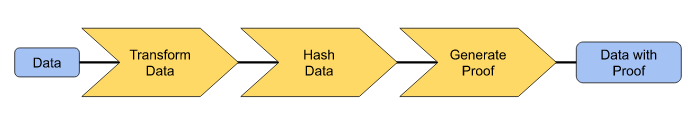
\includegraphics[width=1\textwidth]{Images/c5_1.png} 
  \caption{Process to create a cryptographic proof.}
\end{figure}

Next, verifying the proof requires three steps to be completed \cite{VCDataIntegrity}. The initial steps comprise the Transformation and Hashing processes which were previously presented, 
followed by the Cryptographic Proof Verification which involves some specific algorithms that confirm the reliability of the data being put in. It could mean checking up 
on the validity of digital signatures or verifying participation proofs.

\begin{figure}[h]  
  \centering
  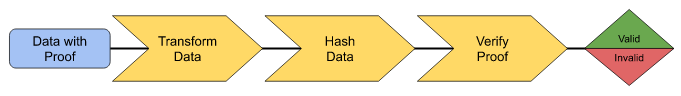
\includegraphics[width=1\textwidth]{Images/c5_2.png} 
  \caption{Process to verify a cryptographic proof.}
\end{figure}

\subsubsection{Proof Data Model}

A data integrity proof in \gls{ssi} systems consists of a number of parameters, some mandatory and some optional; among the first ones there are \cite{VCDataIntegrity}: 

\begin{itemize}
  \item \textbf{Type}: Identifies the exact proof type for cryptographic proof, thus, allows the relevant fields that are used to validate and verify the provided proof.
  \item \textbf{Proof Purpose}: Explicates the purpose of the proof, protects against the misuse and guarantees its proper implementation.
  \item \textbf{Verification Method}: Provides a description of the procedure and the data that may be required to verify the proof, which may involve cryptographic proofs 
  or other verification tools.
  \item \textbf{Proof Value}: It contains the encoded binary data that is required for proof verification, which is the process that uses the specific verification method.
\end{itemize}

\begin{figure}[h]  
  \centering
  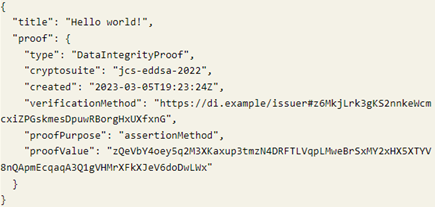
\includegraphics[width=0.8\textwidth]{Images/c5_3.png} 
  \caption{A simple example of cryptographic proof.}
\end{figure}

In addition, other optional parameters can also be included within a proof, such as \cite{VCDataIntegrity}: id, created, expires, domain (useful for representing the security domains in which the 
proof is meant to be used, ensuring its proper application within specified contexts) ,challenge (only if the domain is specific, to mitigate replay attacks), previousProof 
and nonce (useful to increase privacy by decreasing linkability, that is the result of deterministically generated signatures).

\subsection{Digital Signature using EdDSA}

In the manner before, the usage of the approach of digital signature is very common on the way of creating a proof. As a part of different algorithms, one that has the most 
outstanding impact is \gls{eddsa}, which its implementation we will cover in this subsection. Using the elliptic curve cryptography, the \gls{eddsa} is one of the most known for its 
speed and security.

\subsubsection{EdDSA Key Generation}

Key generation in \gls{eddsa} consists in the creation of a private-public key pair. The private key ($priKey$) consists of 32 octets of cryptographically secure random data 
(256 bit). For the public key ($pubKey$) the hashing algorithm (SHA-512) is applied to the private key as the first step in the process. And finally, the hashing product is 
converted using specific bit operations, as well as scalar multiplication, in order to get the public key \cite{10054286}. Specifically, this process involves the following steps:

\begin{enumerate}
  \item \textbf{Hashing}: The first step is hashing the private key (priKey) of 32-byte, using SHA-512, and store the result in a 64-octet buffer denoted as $h'$; only the 
  first 32-byte will be considered for the $pubKey$.
  \item \textbf{Buffer Pruning}: Then, some bit manipulations are performed on the buffer to ensure compliance with specific encoding requirements, for example some specific
  bits are clear in the first and last octets.
  \item \textbf{Scalar Multiplication}: The pruned buffer is then considered as a secret scalar represented by a little-endian integer and a fixed-base scalar multiplication
  $[s']B$ is performed, where $B$ represents a base point on the elliptic curve. 
  \item \textbf{Encoding}: Finally, the resulting point $[s']$ is encoded, through manipulation of the $y$-coordinate values of the curve. In this way the $pubKey$ has also 
  been generated.
\end{enumerate}

\subsubsection{EdDSA Signing}

Signatures are formed by using the private key to sign the message. This process is based on combining the message and the private key by using different cryptographic 
operations \cite{10054286}. In our case, the message corresponds to the value of the proof to be signed. Specifically, this process involves the following steps:

\begin{enumerate}
  \item \textbf{Hashing and Scalar Derivation}: The private key ($priKey$) is hashed using SHA-512 to obtain a digest ($h'$), of which the first half is used to create the 
  secret scalar $s'$, while the second half is denoted as prefix.
  \item \textbf{Message Hashing}: The message ($M'$) is hashed using SHA-512, along with prefix, context information ($CTX$) and a flag ($FLG$), so as to obtain a 64-octet 
  digest ($i$).
  \item \textbf{Point Calculation}: The point $[i]B$ is calculated, where $B$ is the base point on the elliptic curve. This calculation includes the reduction of 
  $i$ modulo $L$, that is, the group order of $B$, and finally the result is encoded, obtaining $R$.
  \item \textbf{Digest Calculation}: Then, another digest is computed by hashing the concatenation of $CTX$, $FLG$, $R$, the public key ($A$), and a modified hash of the message 
  ($PH(M')$), and from this is obtained the little-endian integer $k$.
  \item \textbf{Scalar Calculation}: $S' = (i + k \cdot s') \mod L$ is calculated.
  \item \textbf{Signature Construction}: Finally, the signature is created by concatenating $R$ (32 octets) and $S'$ (32 octets, with the three most significant bits at $0$) 
  in little-endian encoding.
\end{enumerate}

\subsubsection{EdDSA Verify Signature}

Signature verification attests to the authenticity of a certain signature by utilizing the public key, message (in our case the proof), and signature data. This method is 
based on decoding the signature, forming a digest out of the message and public key, and finally, verifying the group equation to ensure the integrity of the signature \cite{10054286}. 
Specifically, this process involves the following steps:

\begin{enumerate}
  \item \textbf{Signature Decoding}: Using the public key $A$ as reference point, the signature is decoded into two 32-octet parts, which represent the point $R$ and integer 
  $S'$, respectively.
  \item \textbf{Digest Generation}: Then, a 64-octet digest is generated by hashing the concatenation of $CTX$, $FLG$, $R$, public key ($A$), and a modified hash of the message 
  ($PH(M')$).
  \item \textbf{Group Equation Verification}: Finally, the validity of the signature is verified by checking the group equation $[8][S']B = [8]R + [8][k]A'$, or 
  alternatively, $[S']B = R + [k]A'$; where $A'$ is the public key encoded.
\end{enumerate}

\section{Cybersecurity within SSI}

\subsection{Security in Blockchain and SSI}

As previously outlined, in the context of \gls{ssi}, blockchain may be used as a distributed ledger to implement certain security features for the system. Nevertheless, this 
might not be sufficient enough because the \gls{ssi} model still contains some vulnerabilities. Next, we present the main features of blockchain technology, useful for the \gls{ssi} 
system, and after that we examine the security challenges according to the security assessment of the \gls{ssi} system. 

\subsubsection{Security Features in Blockchain}

Among the key security features of blockchain, those most crucial for decentralized identity management include \cite{CyberSecurity}:

\begin{itemize}
  \item \textbf{Tamper Resistance}: Data immutability is ensured via blockchain thus cryptographic hashing methods, linking each block cryptographically. Consensus 
  Protocols like Nakamoto consensus and digital signature algorithms such as \gls{ecdsa} mitigate the tampering of data.
  \item \textbf{DDoS Resistance}: The decentralized architecture of blockchains consensus protocols allows the reduction of DDoS attacks' impact, since they permit 
  transaction processing even with offline network nodes. In this scenario, attackers must compromise a significant portion of the network to make it inoperable.
  \item \textbf{Double Spending Resistance}: Consensus protocols and transparent transactions permit the mitigation of double-spending attacks, while verification 
  mechanisms guarantee transaction's validity, maintaining network integrity.
  \item \textbf{\%51 Resistance}: Attacks made against consensus protocols require the attacker to gain majority control, threatening the integrity of the transaction 
  history. Various consensus protocols have different susceptibility thresholds, so several robust security measures must be developed.
\end{itemize}

\subsubsection{Security Assessment of SSI}

The main challenges that \gls{ssi} models must approach are \cite{CyberSecurity}:

\begin{itemize}
  \item \textbf{Dependency on Manufacturer Reliability}: \gls{ssi} systems depend on \gls{tee}s supplied by the manufacturers, which is crucial for 
  the security of the systems. The reliance put on the security model manufacturers come up with is also dubious and might introduce further vulnerabilities associated with 
  single points of failure.
  \item \textbf{Data Availability and Memory Risks}: Storing verifiable credentials in a local storage in the \gls{ssi} systems can decrease the accessibility and can expose 
  issues related to memory corruption or misuse. The availability of the data spot on without ruining the integrity is a big question.
  \item \textbf{Confidentiality Protection and Information Disclosure Risks}: Although \gls{ssi} systems are using different methods such as anonymous authentication and 
  \gls{zkp}s to protect privacy, risks for disclosing sensitive identity information still remain. The reasonable selective disclosure mechanisms are 
  still under development. The implementation of these mechanisms should be improved to mitigate the risks.
\end{itemize}

\subsection{Potential Attacks on the SSI System}

The vulnerabilities identified in the previous segment could give malicious actors the push to conduct different types of attacks and lead to damage or steal identities of other 
people to the \gls{ssi} system. These attacks can be grouped into three categories, and an attack tree can be defined for each of them in order to better analyze them.

\subsubsection{Fake Identity Attacks}

Fake identity attacks pose a major threat to \gls{ssi} systems, using fake identities to gain access to services they are not authorized for. Attackers exploit vulnerabilities in 
the \gls{ssi} architecture to create fake credentials. These attacks can damage the trust and reliability of the identity management system as a whole \cite{CyberSecurity}.

\begin{figure}[h]  
  \centering
  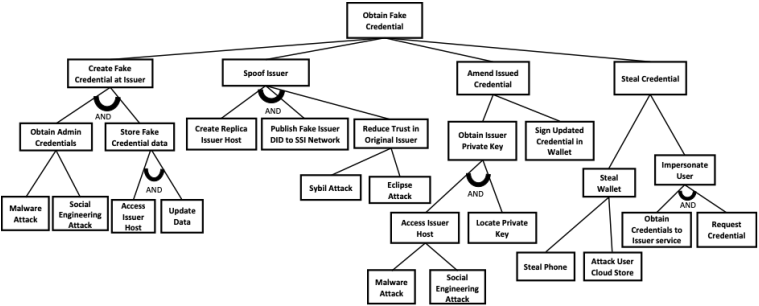
\includegraphics[width=1\textwidth]{Images/c5_4.png} 
  \caption{An attack tree of Faking Identity Attacks in the SSI system.}
\end{figure}

\newpage

\textbf{Attack Tree Analysis}: In this attack scenario, attackers pretend to be trusted issuers by creating fake credentials, like \gls{did}s and public keys. Once inside the 
network, they trick it into believing these fake credentials are real. In addiction, vulnerabilities in the architecture, like hacked network machines, can give attackers 
access to secret administrative credentials and keys, allowing them to change them. For instance, in the Eclipse Attack, attackers take control of the peer-to-peer network 
by redirecting connections to fake nodes, making the network accept the false credentials \cite{9659929}.

\subsubsection{Identity Theft Attacks}

Identity theft attacks use vulnerabilities, in the \gls{ssi} system to steal sensitive and personal information, from user wallets without permission. These actions put 
individuals’ privacy at risk and could result in types of fraudulent activities and improper use of personal data \cite{CyberSecurity}. 

\begin{figure}[h]  
  \centering
  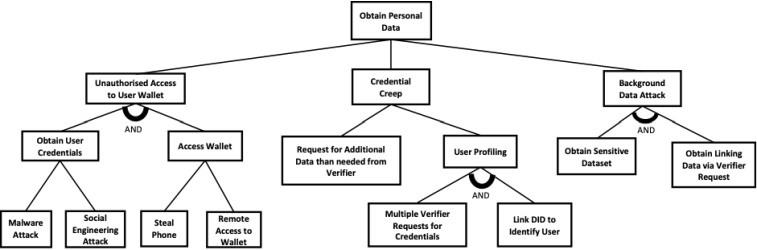
\includegraphics[width=1\textwidth]{Images/c5_5.png} 
  \caption{An attack tree of Theft Identity Attacks in the SSI system.}
\end{figure}

\textbf{Attack Tree Analysis}: In this type of attack, malicious actors might access data in wallets without permission by exploiting vulnerabilities in the \gls{ssi} 
infrastructure. To do that, They could exploit authentication weaknesses or misuse credential verification methods to obtain additional personal information, a practice 
known as Credential Creep. The impact of identity theft attacks goes beyond users impacting the credibility and reliability of the \gls{ssi} environment as a whole \cite{9659929}. 

\subsubsection{DDoS Attacks}

\gls{ddos} attacks pose a serious risk to the availability and reliability of \gls{ssi} system services. Through attacking the system with a large 
volume of traffic, the attackers intend to cripple the users’ access to the system and breach the system’s function \cite{CyberSecurity}.

\begin{figure}[h]  
  \centering
  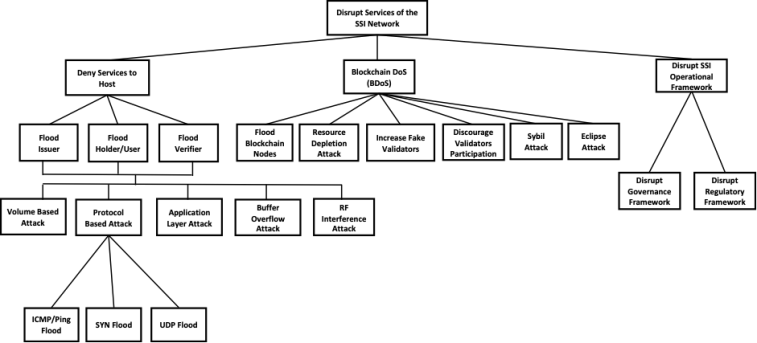
\includegraphics[width=1\textwidth]{Images/c5_6.png} 
  \caption{An attack tree of Distributed Denial of Service Attacks in the SSI system.}
\end{figure}

\textbf{Attack Tree Analysis}: This type of attacks aim at several parts of the \gls{ssi} system, such as issuer, holder, and verifier hosts, along with the distributed ledger nodes. 
Malicious actors can exploit vulnerabilities to attacks using vulnerabilities in the blockchain infrastructure, for example flooding the nodes or disrupting the consensus 
process. Furthermore, operational frameworks can be targeted, leading to difficulties in governance and regulatory processes that are imperative for the functioning of the 
\gls{ssi} ecosystem \cite{9659929}.

\chapter{Design and Implementation} \label{ch:framework}

Once the initial research was completed on the basics of blockchain and the current stage of the development of \gls{ssi} models, the objective of this thesis was developed. The 
first goal is to make the standalone framework for the decentralized user identity management, applying the \gls{ssi} models with the blockchain technology as the foundation. In 
this model, the identity management process consists of authentication and authorization procedures that do not rely on centralized systems or databases. The blockchain 
technology, smart contracts, and \gls{vc}s are used for this purpose. Therefore, it guarantees a high level of seclusion and security for the personal and 
sensitive information of the users.

Subsequently, the aim was to integrate this system into an ongoing project at Links Foundation named Data Cellar. Chapter \hyperref[ch:integration]{7} will delve into what Data Cellar is and discuss 
the integration of the framework into that project. 

In this chapter instead, the work will be analyzed in the design and implementation of the standalone framework for decentralized identity management. The work comprised 
several phases: analysis of existing projects in this domain, selection of the environment and libraries for developing the project, actual implementation of the project, 
and analysis of its limitations arising from the lack of robust support structures not yet commercially available, given the relatively short time since the development of 
blockchain-based \gls{ssi} systems.

\section{Framework Development Journey}

In this section, the design phase of the standalone framework is explored, tracing the journey from initial research to the final selection concerning the development 
environment, namely the blockchain and libraries for managing \gls{did}s. The choices made regarding the management of another fundamental element of the \gls{ssi} model, namely \gls{vc}s, 
will be discussed in section \hyperref[sec:6.3]{6.3}.

\subsection{Initial Research}

Firstly, we conducted an examination of the primary \gls{idms} blockchain products on the market. Several scientific papers and articles were examined to identify their technology
choices, means of operation, and functionalities they offer \cite{9315899}, \cite{9129332}, \cite{8776589}. The three primary solutions encountered were:

\begin{itemize}
  \item \textbf{ShoCard}: This \gls{ssi} technology underlines the decentralization providing every user with full control over their identities and data. \textit{ShoCard} uses the public 
  Bitcoin blockchain for digital identity and authentication, when users hold their identities on their devices using private keys.
  \item \textbf{The Sovrin Network}: Governed by \textit{Sovrin Foundation}, it is an open-source solutions framework that provides users with sovereign and decentralized digital 
  identities. It uses Sovrin ledger as a blockchain to support \textit{Hyperledger Indy} framework and other \textit{Hyperledger} libraries like \textit{Aries} and \textit{Ursa}.
  \item \textbf{The uPort System}: An open-source identity system management with \gls{ssi}. It uses Ethereum blockchain for identity representation and 
  \gls{ipfs} for data storing.
\end{itemize}

\renewcommand{\arraystretch}{1.4}
\begin{table}[h]
  \centering
  \begin{tabularx}{\textwidth}{|>{\centering\arraybackslash}m{3.3cm}|>{\centering\arraybackslash}m{3.2cm}|>{\centering\arraybackslash}m{3.2cm}|>{\centering\arraybackslash}m{3.2cm}|}
    \hline
    \thead{Project} & \thead{ShoCard} & \thead{Sovrin} & \thead{uPort} \\
    \hline
    Blockchain Implementation & Bitcoin & Hyperledger Indy & Ethereum \\
    \hline
    Blockchain Type & Permissioned & Public Permissioned & Permissionless  \\
    \hline
    Storage & Off-Chain & On/Off-Chain & Off-Chain  \\
    \hline
    Interoperability & Yes & Yes & Yes  \\
    \hline
    Selective Disclosure & No & Yes & Yes  \\
    \hline
    Auth & Yes & Yes & No  \\
    \hline
  \end{tabularx}
  \caption{A comparative analysis of blockchain based SSI system.}
\end{table}

In order to avoid the usage of the existing systems and to bring up a decentralized identity management system from scratch, the main work was done on the fundamentals. The 
first step was the creation of a unique user representation that in the case of a decentralized system is ensured by the \gls{did}s. Several libraries facilitating \gls{did} creation 
and management were explored \cite{10218198}, including:

\begin{itemize}
  \item \textbf{Ethr-did}: Utilizes Ethereum's accounts and smart contracts to implement the registry for \gls{did}s resolution. It stores \gls{ddo} on the Ethereum blockchain.
  \item \textbf{Did-algo}: A framework for the \textit{Algorand} blockchain, storing \gls{ddo}s on \gls{ipfs}. It offers a \gls{cli} software for managing operations and supports various 
  cryptographic keys.
  \item \textbf{Did-indy}: Part of the \textit{Hyperledger Indy} ecosystem, based on a permissioned blockchain with multiple logical ledgers. It enables role assignment to \gls{did}s and 
  provides mechanisms for \gls{vc} issuance and verification.
\end{itemize}

\subsection{Challenges and Failed Attempts}

Initially, there were works focusing on the analysis of the \textit{Did-indy}, which is also built on the \textit{Hyperledger Indy} blockchain. Nevertheless, the development was challenged 
by the outdated \textit{Indy} \gls{sdk} and the absence of the comprehensive guideline. 

These constraints thus provoked an exploration of other solutions, which resulted in a focus on \textit{algo-did}, which works on the \textit{Algorand} blockchain. It turns out that 
there were certain challenges that we encountered with \textit{algo-did}, such as documentation issues, technical problems that remain unresolved, and the lack of community 
support that we have noticed. These problems led to a re-evaluation of the relevance of this system for the framework.

\subsection{Final Choice}

After a thorough screening and exclusion process, the spotlight focused on \textit{ethr-did}, which is based on the Ethereum blockchain, one of the most widely used blockchains at 
present. The \textit{ethr-did} system was not only robust but also well-documented, and \textit{uPort} also made use of it, as discussed before, which made it the ideal option. 

In the beginning, the \textit{ethr-did} library's functionality was tested by running locally executed software, using \textit{Infura} to communicate with the Ethereum blockchain. 
Developers can easily get access to the blockchain networks through \textit{Infura} by creating an \gls{api} key, and this is done without requiring them to directly manage 
full nodes on their devices \cite{infura}.

However, anticipating the integration of the framework with the Data Cellar project, envisioned as a browser-accessible application for users, the framework was promptly developed 
in the form of a browser \gls{dapp} supported by the use of MetaMask. MetaMask serves not only as a digital wallet for users but also facilitates direct communication with the 
blockchain through the browser, eliminating the need for an \gls{api} key and thus \textit{Infura}.

\section{Framework Main Components}

In this section, the libraries, blockchain, and support tools utilized in the development of the standalone framework designed as a browser \gls{dapp} for 
identity management will be explored. This framework operates under the decentralized identity management model based on blockchain technology, focusing on the creation and 
management of \gls{did}s. The section excludes the management of \gls{vc}s, which will be addressed in the subsequent section.

\subsection{Ethr-did and Other Libraries}

The foundation for standalone framework development is \textit{ethr-did} library. Through \textit{ethr-did}, we try to use Ethereum addresses as a fully self-directed \gls{did} 
so as to help easy key development and management for these identifiers. \textit{ethr-did} standardizes the identity methods and provides a scalable mechanism for 
public keys and Ethereum addresses \cite{ethr-did}. Thus, the collection of on-chain and off-chain data becomes possible. 

This library relies on two additional libraries: 

\begin{itemize}
  \item \textbf{ethr-did-registry}: This library contains the Ethereum contract code allowing owners of \textit{ethr-did} identities to update attributes in their \gls{ddo}s. 
  It provides an \gls{api} enabling developers to interact with the contract functions using JavaScript, designed for resolving public keys for off-chain authentication \cite{ethr-did-registry}.
  \item \textbf{Ethr-did-resolver}: Intended for use with Ethereum addresses or secp256k1 public keys as fully self-managed \gls{did}s, wrapping them in a \gls{ddo}. It 
  supports the \gls{did}s spec from the W3C Credentials Community Group and relies on the \textit{did-resolver} library \cite{ethr-did-resolver}.
\end{itemize}

\textit{ethr-did} together with \textit{ethr-did-registry} and \textit{ethr-did-resolver} are all based on \textit{ethers}, which is a thin and well-known library for smart contract interactions and 
\gls{dapp}s development, most commonly used for digital wallets, like MetaMask.

The other hand, \textit{ethr-did} makes use of the \textit{did-jwt} library thereby introducing the signing and verification of \gls{jwt}s using various algorithms. However, specific 
functions from \textit{did-jwt} were not utilized in the framework created. 

In this case, only the \textit{ethr-did} constructor was used to generate \gls{did}s associated with users' Ethereum accounts and resolved them later using the \textit{ethr-did-resolver} library. 
Supplementary functions within \textit{ethr-did} were unnecessary for the purposes and thus remained unused.

\subsubsection{Ethr-did Constructor}

The majority of functions within the \textit{ethr-did} library can be executed either locally or interact directly with the Ethereum blockchain, depending on the chosen approach for 
constructing the \textit{ethr-did} object, whether or not the etherDidController class from the \textit{ethers} library. 

Now, let's analyze in detail the parameters required by the constructor \cite{ethr-did}: 

\begin{itemize}
  \item \textbf{identifier}: Represents the identifier used for \gls{did} creation, which can be either an Ethereum address, a public key, or an Ethereum address as a string. (Required)
  \item \textbf{chainNameOrId}: Represents the name or ID of the blockchain network. (Optional)
  \item \textbf{registry}: Represents the address of the \gls{did} registry contract. (Optional)
  \item \textbf{signer}: Represents the \gls{jwt} signer. (Optional)
  \item \textbf{alg}: Represents the signature algorithm, which can be either 'ES256K' or 'ES256K-R'. (Optional)
  \item \textbf{txSigner}: Represents the transaction signer. (Optional)
  \item \textbf{privateKey}: Represents the private key associated with the Ethereum address. (Optional)
  \item \textbf{rpcUrl}: Represents the RPC URL used to connect to the Ethereum network. (Optional)
  \item \textbf{provider}: Represents the Ethereum provider. (Optional)
  \item \textbf{web3}: Represents the web3 provider. (Optional)
\end{itemize}

The constructors logic checks, for the existence of an Ethereum provider or network details. If present, sets up the \textit{txSigner} using an object that can sign transactions or 
generates one, from a \textit{Wallet}. If a private key is defined and theres no existing \textit{txSigner} object a fresh \textit{Wallet} object is generated with the given key, which is then 
utilized as the \textit{txSigner} for signing transactions.

The \textit{EthrDidController} class is created to work with the ERC1056 contract, which's a standard used to represent identities, on the Ethereum platform. When the \textit{EthrDid} 
object constructor is called it triggers the constructor of \textit{EthrDidController} generating a \gls{did} with \textit{did:ethr} on the designated network, in a process. This means that only 
\gls{did}s generated through \textit{EthrDidController} and actions executed using its functions are able to communicate with the Ethereum network.

\subsection{Ethereum and Smart Contracts}

As previously mentioned, for the purpose of building the following framework of decentralized identity management, the Ethereum blockchain has been chosen. Ethereum is 
possibly one of the most widely used blockchains in the world today due to the fact that it has completely redefined the concept of blockchain itself through the functions 
of smart contracts and through the support for the development of \gls{dapp} \cite{ethereum}.

In particular, Ethereum's main test networks, namely \textit{Goerli} and \textit{Sepolia}, were used, given the possibility of obtaining the relevant tokens via faucets. A smart contract was 
set up on these blockchains to serve as a registry, for keeping track of which \gls{did}s linked to users Ethereum accounts had registered on the browser \gls{dapp}. In 
addition, the smart contract used by \textit{ethr-did} for managing \gls{did}s, which is useful during their resolution, already present on \textit{Goerli}, has also been 
deployed on \textit{Sepolia}.

Deployment of these contracts on \textit{Goerli} and \textit{Sepolia} will be facilitated by using \textit{Truffle}, a development framework for Ethereum that eases and hastens the creation of smart 
contracts and \gls{dapp}s. After correctly configuring \textit{Truffle} \cite{truffle-suite}, a brief script was created to deploy the contract, using the following commands: 

\begin{itemize}
  \item \textbf{"truffle compile"}: to compile the contract and obtain the \gls{abi}, which describes the methods it accepts, the parameters they accept, and the values returned.
  \item \textbf{"truffle migrate --network"}: to deploy the contract correctly on the given blockchain network, provided that the account used has enough tokens to cover 
  the fees. During deployment, the address of the block where the contract had been stored on the blockchain was retrieved.
\end{itemize}

\newpage

\lstinputlisting[language=JavaScript, caption={Deploying DataCellarRegistry contract.}]{Codes/deploy.js}

\subsubsection{The Smart Contract}

A smart contract is a self-executing contract wherein the conditions of the agreement are automatically captured in code. It executes the agreement conditions automatically 
and intermediaries are no longer a necessity. 

In the scope of the project, Solidity language is used to write a smart contract that will perform functions of user registration management in a decentralized way. It is 
realized by updating a mapping in which a boolean value is attached to each Ethereum account to show the user status whether he is registered or not. In using the Ethereum 
blockchain which is inherently decentralized and immutable, the Smart contract ensures the integrity and transparency of the system, while eliminating the need for a central
authority. Participants can register or unregister themselves safely and autonomously, with the contract recording these actions on the blockchain. 

Functions of the smart contract:

\begin{enumerate}
  \item \textbf{registerUser(address \_userAddress)}: It registers a user in the registry. This function can only be called by the user, and the user must not be already registered.
  \item \textbf{unregisterUser(address \_userAddress)}: Unregisters the user. This function can be called only by the user itself, and the user should have registered before that.
  \item \textbf{isUserRegistered(address \_userAddress)}: Checks if a user is registered in the registry. This function can be used by anyone, and it returns a boolean 
  value indicating whether the user is registered or not.
\end{enumerate}

The contracts three functions all require an Ethereum account as input. The final function is read only displaying whether a user is registered or not while the other two 
functions alter the contracts state. These state altering functions need the contract to update its status on the blockchain leading to transaction fees being paid to 
miners for overseeing and validating these modifications.

\lstinputlisting[language=Solidity, caption={Smart contract for DataCellarRegistry.}]{Codes/registry.sol}

\subsection{MetaMask}

One of the crucial factors that led to the construction of the framework as a browser \gls{dapp} is MetaMask. MetaMask is a user-friendly Ethereum blockchain software 
wallet designed for convenient transaction operations \cite{metamask}. In other words, MetaMask serves as an interface between the users and Ethereum \gls{dapp}s, providing access to Ethereum 
wallets via browser extensions or mobile applications. The advent of MetaMask has provided users with a convenient way to manage their cryptocurrencies, transact online, 
and engage \gls{dapp} across different browsers and mobile platforms. 

Specifically, the browser \gls{dapp} is able to monitor the presence of the MetaMask extension in the browser being used and the existence of an Ethereum 
account in the wallet, which most of the time means that the extension is connected to the application. Additionally, the \gls{dapp} can identify the primary account and the 
desired reference networks on MetaMask in real-time. As a matter of fact, MetaMask not only help in handling multiple accounts but also multiple network like \textit{Goerli} and 
\textit{Sepolia} which has been deployed the smart contract.

Finally, MetaMask provides the ability to securely store the private keys of \gls{dapp} accounts in a secure wallet, allowing users to sign and execute transactions that will 
enable them to register or deregister without the private keys ever leaving the extension in clear or encrypted form.

\lstinputlisting[language=JavaScript, caption={Function for updating wallet and accounts.}]{Codes/mm.js}

\section{Verifiable Credentials and Limitations} \label{sec:6.3}

As outlined in section \hyperref[sec:4.3]{4.3}, \gls{vc}s are crucial, in the \gls{ssi} model. So, once the blockchain and libraries for \gls{did} support were determined, the focus of the 
research turned to finding for managing, issuing, and verifying \gls{vc}s.

\subsection{Utilization and Challenges}

The idea was to make dual use of \gls{vc}s within the \gls{ssi} framework: first, to obtain user information certified by an entity, and then, having obtained this information, to 
create a \gls{vc} issued and signed by the browser \gls{dapp}, with a triple purpose:

\begin{itemize}
  \item Ensuring that the user has registered in the registry on the blockchain, i.e., the smart contract uploaded to \textit{Goerli} and \textit{Sepolia}, through the browser \gls{dapp}.
  \item Maintaining the information provided by the user within an immutable credential, being signed by the browser \gls{dapp}.
  \item Allowing the user to present the \gls{vc} issued by the \gls{dapp} to other entities to demonstrate registration with the service.
\end{itemize}

In this way, the user could authenticate the browser \gls{dapp} just if they offer the \gls{vp} related to the \gls{vc} issued by the \gls{dapp} itself, from which the data will be 
read and the user would be allowed to perform certain actions, such as based on age, country of origin, or profession. Furthermore, all of this is carried out in a fully 
decentralized way, which means that the browser \gls{dapp} contains no centralized database which stores the user's sensitive information. The \gls{vc} is the one maintained by 
the user, and then it is temporarily stored in a session cookie to allow them to perform certain functions once authenticated.

However, even though the concept is well founded and aligns completely with the standards outlined by the state of the art of the \gls{ssi} model, two significant challenges 
emerged. These limitations arise from the absence of frameworks and resources, for overseeing and upholding these \gls{vc}s:

\begin{itemize}
  \item The absence, for now, of \gls{vc}s issued by genuine certified entities, easily findable and provided by the user during the registration phase to allow the creation of 
  the \gls{vc} issued by the browser \gls{dapp}. For example, there is currently no \gls{vc} corresponding to an identity card issued by the Italian government or similar
  entities. This limitation forced the direct request to the user to manually enter their data via a form, which is automatically taken as "trusted" and inserted into the 
  \gls{vc} that will be issued.
  \item The absence of non-proprietary wallets capable of storing and managing \gls{vc}s for different purposes and containing \gls{did}s with any type of \gls{did} method. Such wallets are 
  necessary to allow the user to securely store the \gls{vc} provided and to present a \gls{vp}, signed by them and containing only the necessary information requested. This limitation 
  forced the direct request to the user for the \gls{vc} provided, without being able to apply the concept of selective disclosure.
\end{itemize}

\subsection{Solution Exploration}

Another idea that emerged due to a possession of the MetaMask as a wallet for the Ethereum accounts of our users was \textit{Masca}. \textit{Masca}, being a MetaMask Snap (extension), adds 
support for decentralized identity management of \gls{did}s, storage of \gls{vc}s, and creation of \gls{vp}s \cite{masca}. 

This framework appeared to be suitable for the requirements; however for \gls{vc} creation and signing, \textit{Masca} must use the MetaMask account of the user connected to the 
\gls{dapp} browser at that time. By the default mechanism, it was not possible to designate one particular account as an issuer that could have represented an application. 
The only possible way to deal with the problem after contacting \textit{Masca} Support on dedicated forums was to pass the \gls{vc} payload from the user to the server, at which point it 
would be temporarily stored. Later, the application administrator would use another \gls{dapp} to access the requests from the server and sign them, which in turn create the \gls{vc} to be 
finally transmitted to the user via other means. 

However, this solution was disregarded because it not only prohibited immediate user registration and authentication within the application but also necessitated the 
implementation of database within the service, thus eliminating the complete decentralization of the system.

\subsection{Final Decision}

The ultimate choice in this case relied on sending the \gls{vc} from the browser \gls{dapp} to the user, where it is saved on the users device along with a suggestion to keep it 
safe in a place, like a wallet if possible.

In terms of selecting a library to use for \gls{vc} creation and verification, the library \textit{did-jwt-vc} was selected. This library, also used by \textit{Veramo}, the current implementation 
of \textit{uPort}, has \gls{api}s such that they allow for the creation of a \gls{vc} by sending a payload that contains the user's account-associated \gls{did}, along with that of the issuer, that 
is EtherDid object which represents the browser \gls{dapp} \cite{did-jwt-vc}. The process of signing and verifying \gls{jwt}s using the ES256K and \gls{eddsa} mechanisms, respectively, is accomplished 
via the invocation of the functions present in the \textit{did-jwt} library.

Subsequently , the \gls{vc} can be validated by a \textit{Resolver} object that allows the resolution of the \gls{ddo}. Inside \gls{ddo} there are verification methods which contain 
the issuer of \gls{vc}.  These methods are extracted and used for the verification of the signature.  Signature verification provides the assurance that the \gls{vc}'s signature 
complies with the public key that is related to the verification method. All these operations are invoked through calling for the functions within \textit{did-jwt} library.

\lstinputlisting[language=JavaScript, caption={Function for verifying verifiable credentials.}]{Codes/verifyVC.js}

\section{Application Functionality Analysis}

Let us now look in detail at how the standalone \gls{ssi} framework, which was created for decentralized identity management, was built, following the blockchain-based \gls{ssi} model, 
its functionality and the mechanisms it uses. As mentioned earlier, the framework was developed as a browser \gls{dapp}, consisting of a frontend, developed with 
\textit{React}, and a backend, built using \textit{JavaScript}, which serves as the \gls{dapp} server. 

In addition, to solve problems with the secure storage of authentication tokens, within session cookies, the application is supported by \gls{https}. To do this, \textit{OpenSSL} and 
\textit{mkcert} were used to generate \gls{ssl} certificates, which are required to enable \gls{https} functionality. Thus, this enhancement also allowed the overall security 
of the framework to be strengthened, aligning with established best practices for web application development.

\lstinputlisting[language=JavaScript, caption={Handling cookie and setting authentication state.}]{Codes/cookie.js}

In the frontend, which corresponds to the most substantial part of the browser \gls{dapp}, in addition to the complete manage the graphical user interface, 
the user authentication process is also managed, also taking advantage of MetaMask support. This process consists of 3 steps: \textit{Access} (or connection), \textit{Sign up} and \textit{Sign in} (or
authentication). For each of them a different web page has been defined and within each there is always an "information" button that explains to the user what exactly he
has to do at that precise moment. 

Below, in the remaining subsections, the server's functions first and then each step of the authentication process within the frontend, will be examined in detail.

\subsection{Server Implementation}

Being decentralized, the \gls{dapp} server does not contain any database. However, it performs two important functions:

\begin{itemize}
  \item Generating the \gls{vc} with the payload provided by the user and signed with the private key of the application administration, stored as an environment variable within 
  a .env file, during the registration phase of a new user.

  \lstinputlisting[language=JavaScript, caption={Async function for generating JWT token.}]{Codes/createJWT.js}

  \item	Creating and signing, using a secret also stored as an environment variable within the .env file, a \gls{jwt} to be inserted into the session cookie. 
  This \gls{jwt} contains the user's data, which was contained in the \gls{vc} issued to him, which he has to replenish during the authentication phase. The purpose of the \gls{jwt} is to 
  grant specific permissions to the user, based on the data in it, during that session. In addition, before doing so, a check is made on the correctness of a \gls{nonce}, 
  which is signed by the user, within a message, during the authentication phase. This allows to increase the security level of the process itself, preventing replay attacks.

  \lstinputlisting[language=JavaScript, caption={Async function for generating verifiable credentials.}]{Codes/createVC.js}

\end{itemize}

\subsection{Access Process}

Upon launching the framework, the user will be presented with a single button that will redirect them to the page where they can perform the installation of the MetaMask 
browser extension, which is essential for the proper functioning of this \gls{ssi} framework, as it allows users to interact with the blockchain by signing transactions directly 
through their wallet.

Once MetaMask is installed, this one button will be replaced by another that will allow the user to connect the MetaMask extension, to the \gls{dapp} and unlock the wallet,
in case it is still locked, thus allowing the \gls{dapp} to access the Ethereum accounts within it, representing the user.

After doing so, the user will be in the Home of the \gls{dapp}, but will have logged in as a visitor, so they will only be able to view certain parts of the \gls{dapp} 
and perform only limited functions.

However, two buttons will appear in the navigation bar: one for accessing the \textit{Sign in} page and one for the \textit{Sign up} page. In addition, two text boxes will appear showing the 
network and account selected at that particular time, within the MetaMask extension, providing the user with real-time information about the blockchain and the address they 
are working with.

\begin{figure}[h]  
  \centering
  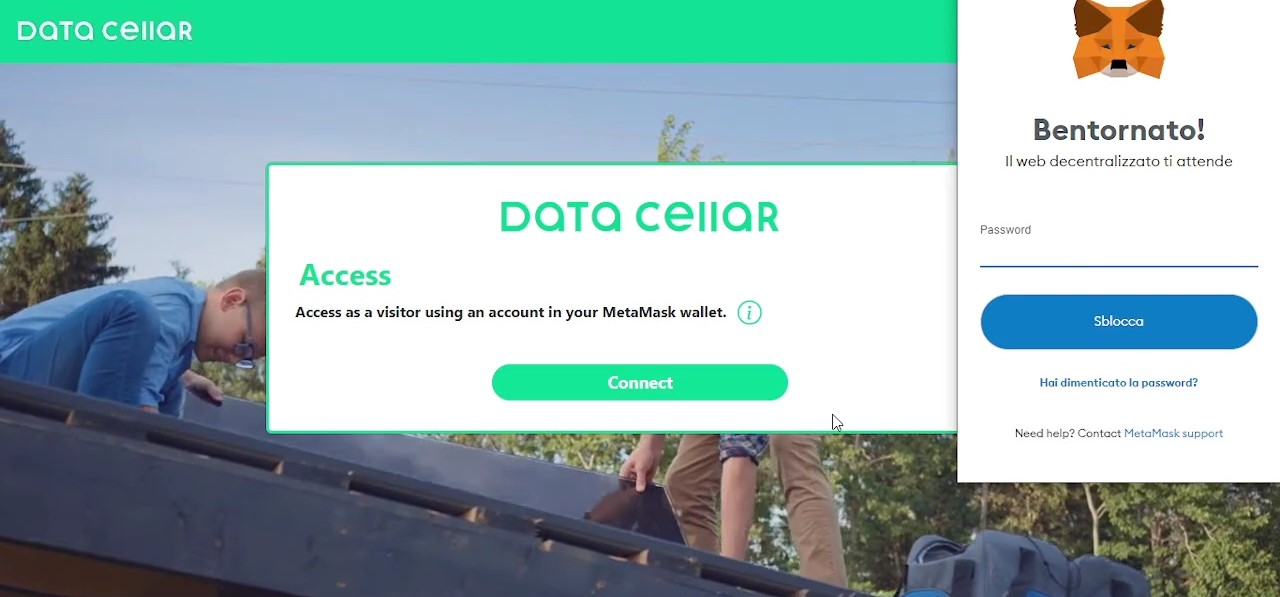
\includegraphics[width=1\textwidth]{Images/c6_1.jpg} 
  \caption{Access page with MetaMask installed.}
\end{figure}

\subsection{Sign-Up Procedure}

This step in the process allows the user to register with the selected account within the MetaMask wallet and using one of the blockchains, in which the smart contract that 
serves as the registry for the \gls{dapp} has been previously deployed.

To begin, the user must fill in all the fields on the form presented to him; every value entered by the user is properly validated, so as to prevent possible security 
problems, but this still does not fully follow the \gls{ssi} paradigm. This is because there are currently no authentic \gls{vc}s from which to take this data (as 
explained in detail in the previous section). This data will constitute the \gls{vc} payload, which the \gls{dapp} browser, in the manner described above, will send through the 
server to the user.

Before receiving this \gls{vc}, however, the user must register by adding his account in the \gls{dapp}'s smart contract, which serves as a registry, present on the referenced 
blockchain. To do so, he must make a transaction, via the MetaMask wallet, which will involve payment of fees, both from MetaMask and from the network used. This 
registration is necessary not only to allow the application administrator to know how many users are registered and with which accounts, but also to control and issue only 
one \gls{vc} per account.

\lstinputlisting[language=JavaScript, caption={Async function for signing up in DataCellar.}]{Codes/register.js}

Once the registration is completed, the \gls{vc} will be provided to the user who, at the push of a button, can download it to his device and store it securely, as indicated.

\begin{figure}[h]  
  \centering
  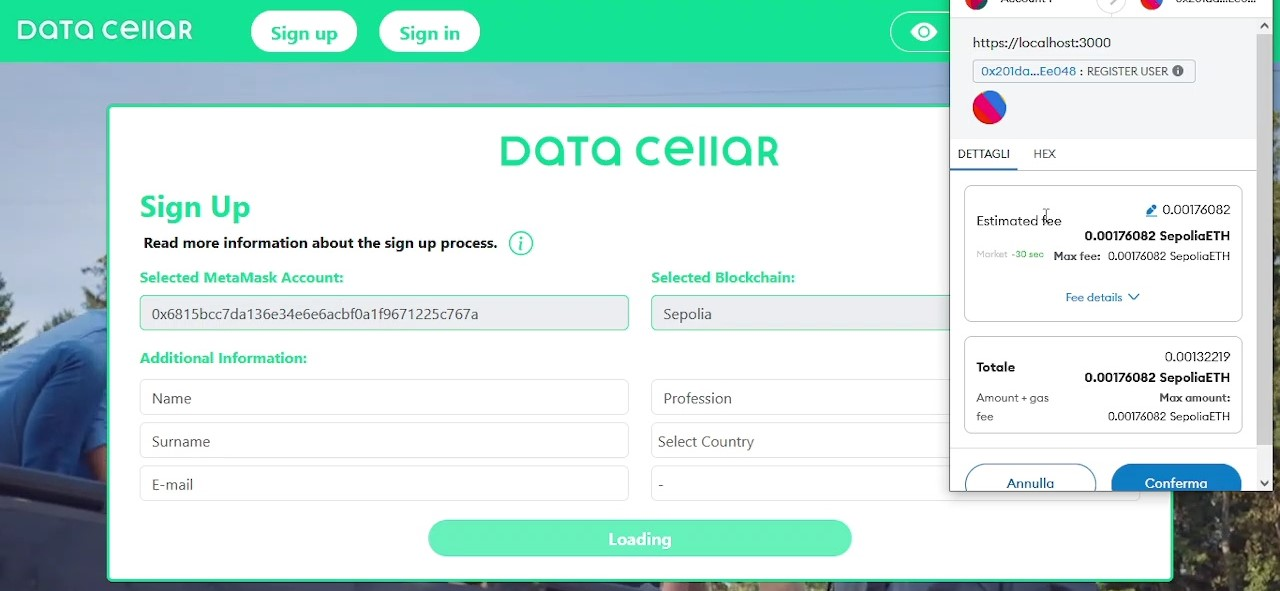
\includegraphics[width=1\textwidth]{Images/c6_2.jpg} 
  \caption{Sign Up page with confirm transaction pop-up.}
\end{figure}


\subsection{Sign-In Mechanism}

In this final and perhaps most important step, user authentication occurs, using the account selected within the MetaMask wallet and the blockchain with which the 
registration was made. A note reminds the user to change the network selected in the MetaMask extension in case it is incorrect.

To do this, the user must provide the \gls{vc} issued during the sign up phase, from the browser \gls{dapp}, for the selected Ethereum account; this is because there is 
currently no way to request the corresponding \gls{vp} (as explained in detail in the previous section). The \gls{dapp} will then check the validity of this \gls{vc}, following the 
methods described above, to ensure both that it has been issued by the \gls{dapp} and that it contains the \gls{did}, associated with the account selected by the user, in his 
MetaMask wallet, at that time.

\lstinputlisting[language=JWT, caption={Verifiable Credential JSON data.}]{Codes/vc.jwt}

If these checks are passed, the user will be asked to sign a message containing a \gls{nonce}, using the private key associated with their account, through the MetaMask wallet. 
This process does not involve any transactions on the blockchain and therefore does not require payment of fees. As explained earlier, this \gls{nonce} serves to increase the 
level of security and will be automatically sent to the server along with the signed message and the payload extracted from the \gls{vc} previously provided by the user. After 
appropriate verification, if successful, the server will return a signed \gls{jwt} containing the payload received.

Finally, this \gls{jwt} will be placed in a token in the session cookies and the user will be authenticated. This corresponds to accessing the \gls{dapp} as a member. In this 
way, the user can view the entire browser \gls{dapp}, access its page, and perform all functionality, within the limits of the information in the session cookies. In fact, 
depending on the functionality the user wishes to perform within the \gls{dapp}, the session cookie token will be decoded and, based on the information obtained, certain 
authorizations will be granted or denied to the user. In addition, a button will appear in the navigation bar that allows the user to log out of the account with which they have authenticated.

\begin{figure}[h]  
  \centering
  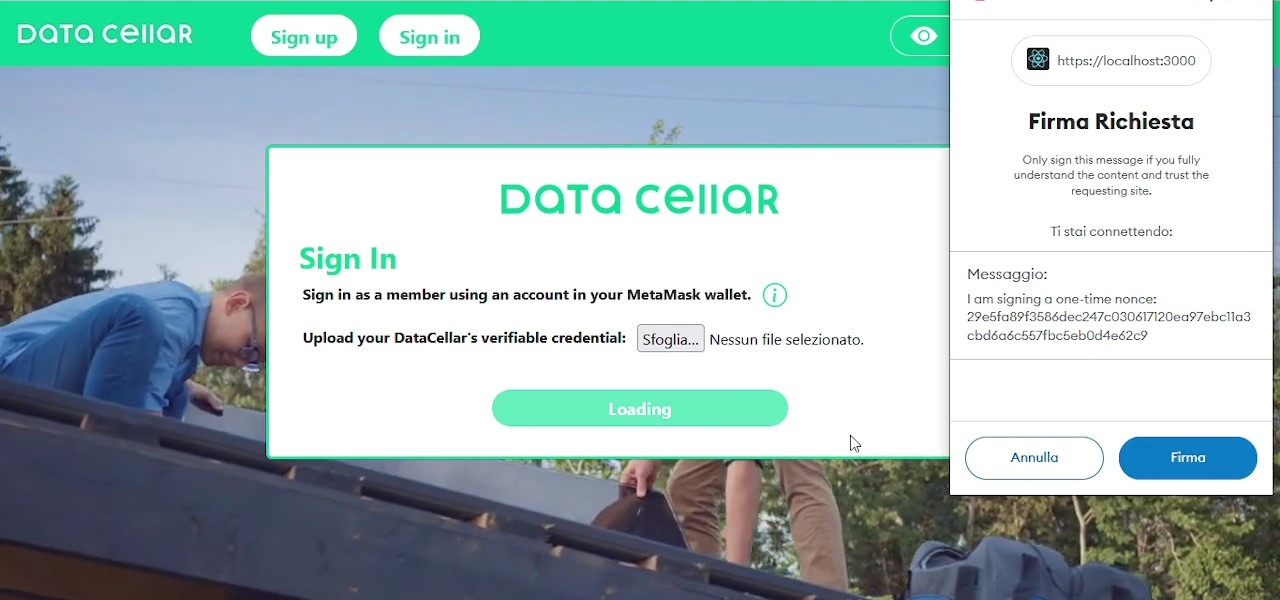
\includegraphics[width=1\textwidth]{Images/c6_3.jpg} 
  \caption{Sign In page with sign message pop-up.}
\end{figure}



\chapter{Integration in a Real Project} \label{ch:integration}

To demonstrate the real utility and effectiveness of the previously created decentralized identity management \gls{ssi} framework, it was integrated as an authentication process 
into an ongoing project at Links Foundation, known as \textit{Data Cellar}. Later, in addition to the integration of this system, the entire \gls{gui} of the application was also developed.

In this chapter, we will first deal with what \textit{Data Cellar} is and what the initial state of the project was. Then, we will examine in detail the entire integration process 
and the final graphical result of the application.

\section{Overview of Data Cellar}

\textit{Data Cellar} is an energy data center, geographically located within the European Union, whose main activities consist of the construction of a federated energy data space in 
order to enable the creation, growth, and support of local energy communities \cite{datacellarproject}. That initiative is based on an innovative rewarded private metering approach,, stressing 
successful integration, simplicity of the interactions, guaranteeing integration with other energy data spaces in the \gls{eu} and providing the actors with the services and tools
they need for their own actions.

As part of this four-year project, Links Foundation endeavors to decentralize various functionalities of the data center, resulting in enhanced security, speed, 
distribution, and additional benefits inherent to blockchain and decentralized architectures.

Naturally, being a project in development within the company and at the outset of this process, in its initial version, the set of functionalities offered by this 
decentralized version is still limited compared to its standard operational version at the European level.

\section{Initial Project Status}

In its decentralized application form, the \textit{Data Cellar} project comprised a set of smart contracts enabling various functionalities (briefly discussed later), invoked through
a backend written in \textit{NestJs}, with its interface generated via \textit{Swagger}. \textit{Swagger}, which is an \gls{api} documentation tool, streamlines the documentation of RESTful \gls{api}s, so that 
the developers could focus on the code while not bothering about the manual creation of documentation.

\subsection{Development Environment}

The execution environment of the project was simulated using \textit{Docker}. \textit{Docker} is an open-source platform that is used for application creation, distribution, and execution, 
all within containers. \textit{Docker} containers represent a modern form of virtualization that allows developers to bundle applications and all their dependencies (such as 
libraries, frameworks, and other components) into a self contained unit known as a "container" \cite{docker}.

Specifically, in this case, three containers were executed: 

\begin{itemize}
  \item \textbf{Ganache:} An Ethereum-based private blockchain simulation containing pre-created accounts with visible private keys and a fund of 100 ETH.
  \item \textbf{Postgres:} The off-chain database for storing user information.
  \item \textbf{Redis:} The service for initializing and using queues to handle requests on the blockchain.
\end{itemize}

As can be seen from these containers, the user identity management system was still completely centralized, using a database implemented through \textit{Prisma}, in which user IDs, 
accounts and private keys were stored.

\subsection{Offered Functionalities} 

The key aspect of the initial version of the project was the digitization of energy data and its exchange among users through the purchase of one-time and periodic licenses.
Features offered included:

\begin{itemize}
  \item User registration, which includes the assignment of an address to the new user enabling them to buy and sell digital assets on the blockchain. 
  \item Visualization of datasets and associated licenses. 
  \item Upload of datasets and associated licenses. 
  \item Purchase of licenses associated with datasets.
  \item Deletion of licenses associated with datasets and the datasets themselves.
  \item Visualization of DataCellar Token balance.
\end{itemize}

\section{Integration Process}

Following the guidelines provided, from the initial version, of the \textit{Data Cellar} project, in the form of a decentralized application, the decision was made to continue using 
\textit{Ganache} as a local network, running through a \textit{Docker} container, rather than using Ethereum testnets, such as \textit{Goerli} and \textit{Sepolia}, as was done for the creation of the 
standalone framework for managing \gls{ssi}.

First, the previously created framework was adapted to work with \textit{Ganache}, and the configuration of MetaMask was then modified. In fact, among other functions, MetaMask 
allowed the addition of new local networks, such as \textit{Ganache}, and the import of corresponding accounts into the wallet. As a final step regarding the blockchain aspect, 
the existing script, which loaded all the contracts used to execute the project's functionalities upon \textit{Docker} startup, had the \gls{ssi} framework smart contract acting as a 
registry and the one used by \textit{ethr-did} for \gls{did} management added.

Subsequently, the code was modified, changing its structure almost completely. This was done because all the \gls{api}s, which invoked the functions, defined within the smart 
contract, had to be moved from the backend, where it was executed only because the users' private keys were stored in plain text in the database, to the frontend, to be 
executed using MetaMask, which allows transactions to be signed without exposing the users' private keys.

During this code change, the use of the database, thus \textit{Prisma} and \textit{Postgres}, the use of queues, as they are not supported by MetaMask, and the use of \textit{Swagger} were completely 
eliminated, as a new \gls{gui} was created.

\section{Final Application}

The second version of the \textit{Data Cellar} corresponds to the final application that has been built, in the form of a decentralized application that has been integrated with the 
SSI framework and is further enriched with a dynamic and user-friendly frontend.

The functionalities of the second version of the \textit{Data Cellar} can be divided into functionalities that relate to the \gls{ssi} framework, those designed for visitors, and those 
for registered members.These functionalities include:

\begin{itemize}
  \item \textbf{SSI functionalities:}
  \begin{itemize}
      \item Connection to \textit{Data Cellar} (log in as a visitor)
      \item Registration to \textit{Data Cellar} (sign up as a member)
      \item Authentication in \textit{Data Cellar} (sign in as a member)
      \item Delete your \textit{Data Cellar} account
  \end{itemize}
  
  \item \textbf{Visitor functionalities:}
  \begin{itemize}
      \item View all datasets available in \textit{Data Cellar}
      \item View all available licenses for each dataset
  \end{itemize}
  
  \item \textbf{Member functionalities:}
  \begin{itemize}
      \item View the balance of ETH and DataCellar tokens
      \item Convert ETH to DataCellar tokens
      \item Add new datasets in \textit{Data Cellar}
      \item Create new licenses, single-use, or periodic, for your datasets
      \item View, edit, and delete your own datasets
      \item View, edit, and delete your own licenses
      \item Buy licenses for datasets added by other users
      \item View purchased licenses and reference datasets
      \item Consume purchased licenses
  \end{itemize}
\end{itemize}

\subsection{Backend Implementation}

To follow the guidelines, provided by the first version of this project, the backend remained written in \textit{NestJs}, using the structure proposed by the language, consisting of 
Module, Controller and Service files. On the logical level, however, within the backend, which acts as a server, only the two features present in the framework for \gls{ssi} 
management remained, namely:

\begin{itemize}
  \item Verification of the user's signature and generation of an access token (which will be placed in the session cookie to verify user authentication)
  \item Generation of a \gls{vc} demonstrating the sign-up to DataCellar (the user must provide it in order to access the dApp)
\end{itemize}

\subsection{Frontend Development}

As in the previous case, the frontend, realized using \textit{React}, covers the most substantial part of the application. It contains not only the entire graphical interface but 
also the authentication process of the \gls{ssi} framework, explained earlier, enriched by the de-registration functionality, along with all the \gls{api}s invoking the functionalities 
defined in the smart contracts of the \textit{Data Cellar} project.

The \gls{gui}, in order to be user-friendly, has been enriched with confirmation modals for the most important operations, which the user can perform, and automatically 
disappearing error and success alerts, which cover all possible outcomes, of the various features the user can perform, within the application.

Finally, let us then briefly examine the two main pages that make up the \textit{Data Cellar} project in its second version in the form of a browser \gls{dapp}. 

\subsubsection{Home Page}

\begin{figure}[h]  
  \centering
  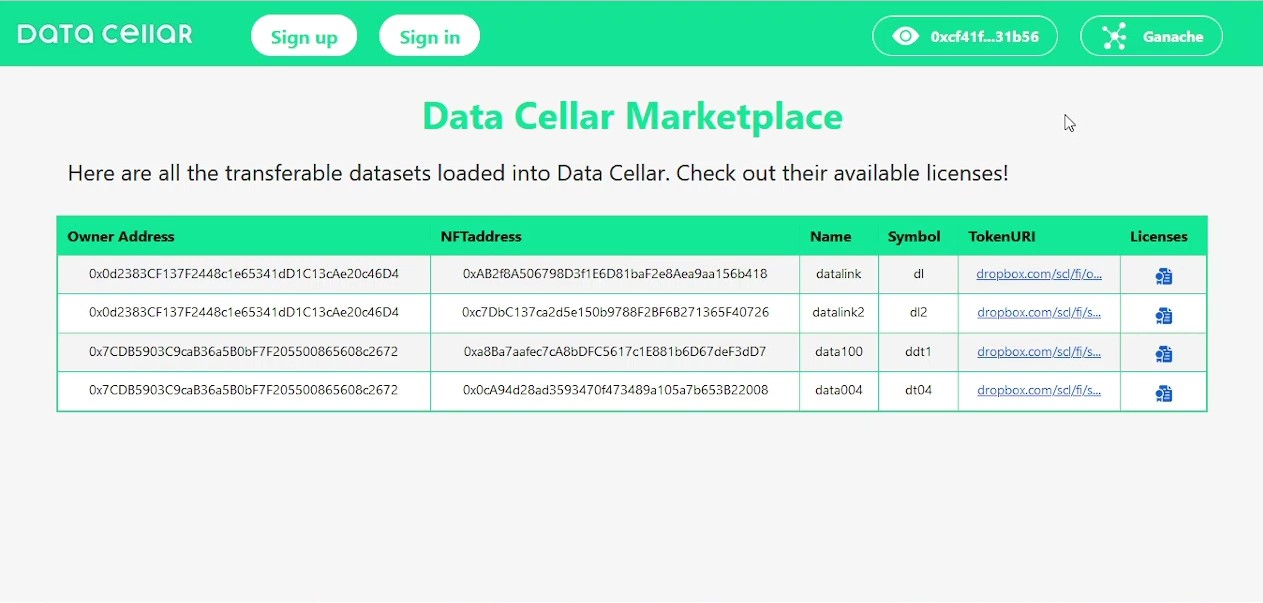
\includegraphics[width=1\textwidth]{Images/c6_4.jpg} 
  \caption{The marketplace in the Data Cellar Home page.}
\end{figure}

The initial page shows the \textit{Data Cellar} marketplace, where all transferable datasets created by other users are visible. Various information is provided for each dataset, 
from the address of the owner, to the \gls{uri} of the Token, which actually contains the energy data.

Clicking on the license symbol takes you to the corresponding page, which shows for the referenced dataset all available licenses, indicating for each of them various 
information, including the price in DataCellar Token, i.e., the currency used within the application. 

\begin{figure}[h]  
  \centering
  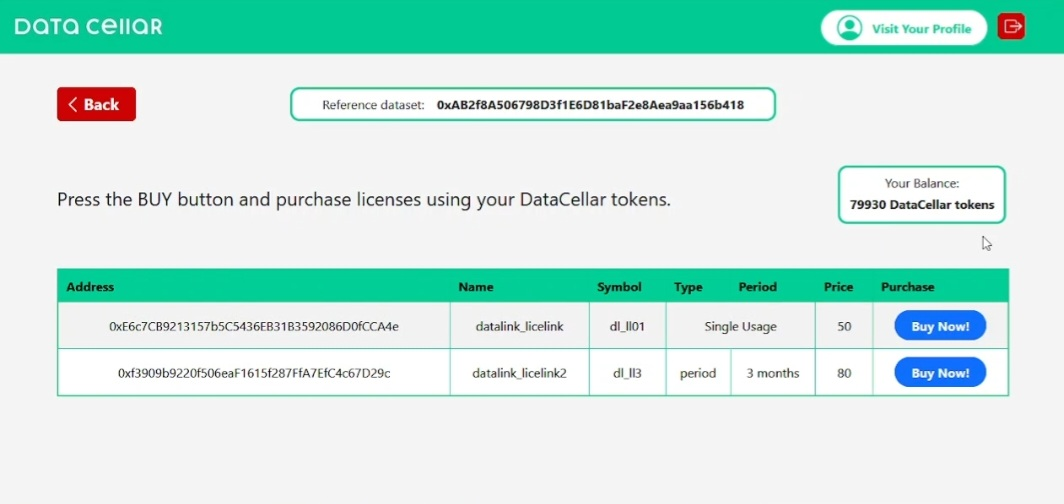
\includegraphics[width=1\textwidth]{Images/c6_5.jpg} 
  \caption{List of licenses for a specific dataset, after authentication process.}
\end{figure}

Authenticated members can purchase these licenses, either for a period or for single use, in the latter case, a modal allowing the definition of the quantity of licenses to
purchase together is provided.

\subsubsection{Profile Page}

By clicking on the "visit your profile" button in the navigation bar, users can access their profile. Within it are various sections covering all the personal functionality 
executable by the user:

\newpage

\begin{itemize}
  \item \textbf{General Information:} Contains the user's information obtained from the token placed in the session cookie.
  
  \begin{figure}[h]  
    \centering
    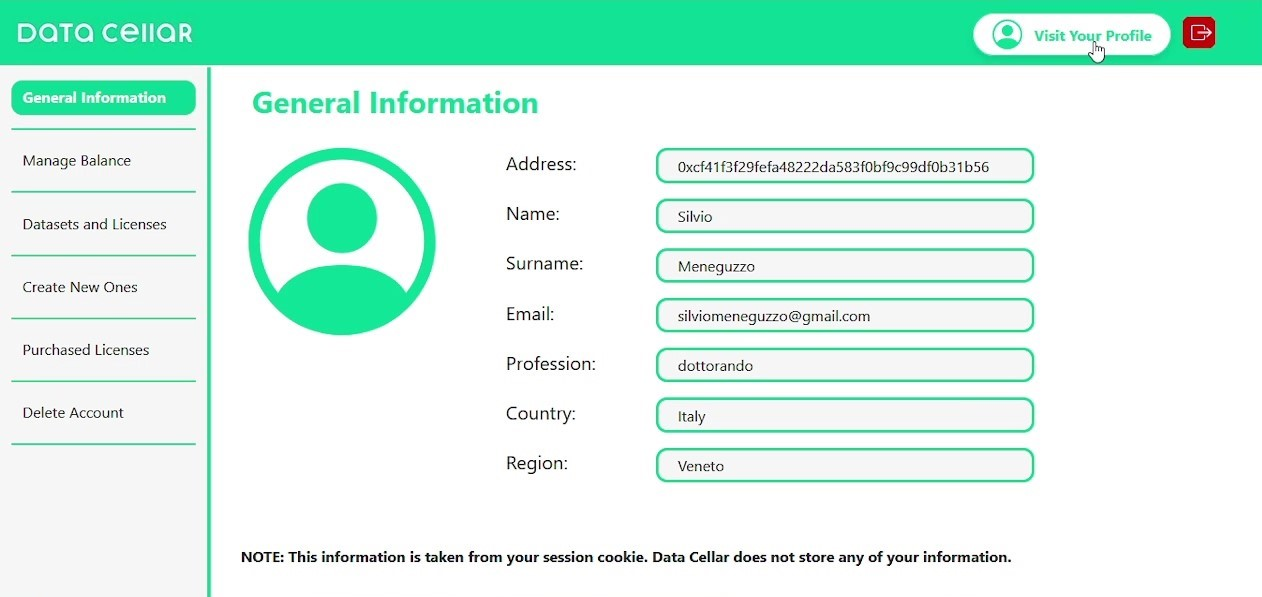
\includegraphics[width=0.8\textwidth]{Images/c6_6.jpg} 
    \caption{Page to view user's personal information.}
  \end{figure}
  
  \item \textbf{Manage Balance:} Displays the user's DataCellar Token and Ethereum balance, also allowing conversion of new ETH to DataCellar tokens.
  
  \begin{figure}[h]  
    \centering
    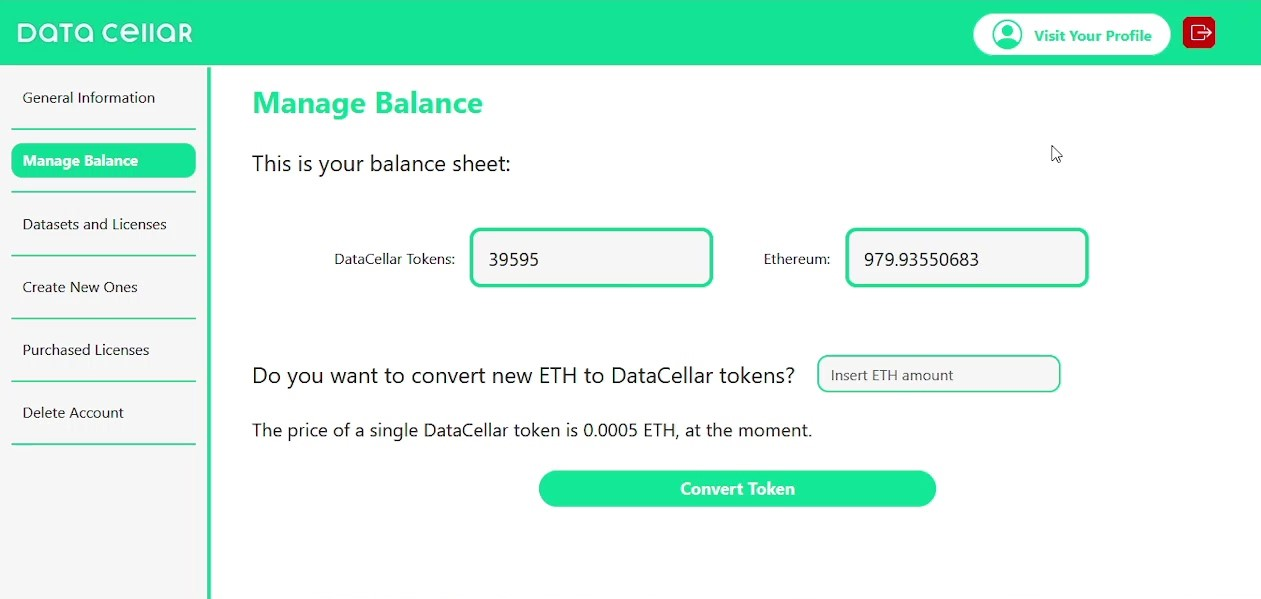
\includegraphics[width=0.8\textwidth]{Images/c6_7.jpg} 
    \caption{Page to manage user's DataCellar tokens.}
  \end{figure}
  
  \item \textbf{Datasets and Licenses:} Displays all datasets created by the user; each can be edited or deleted, using the corresponding buttons that open the relevant 
  modals. Also, by clicking on the license symbols, the user can view all the licenses he has created for that dataset. By accessing the dedicated page, the user can also 
  edit and delete each license through the corresponding buttons and modals, as in the previous case. 
  
  \begin{figure}[h]  
    \centering
    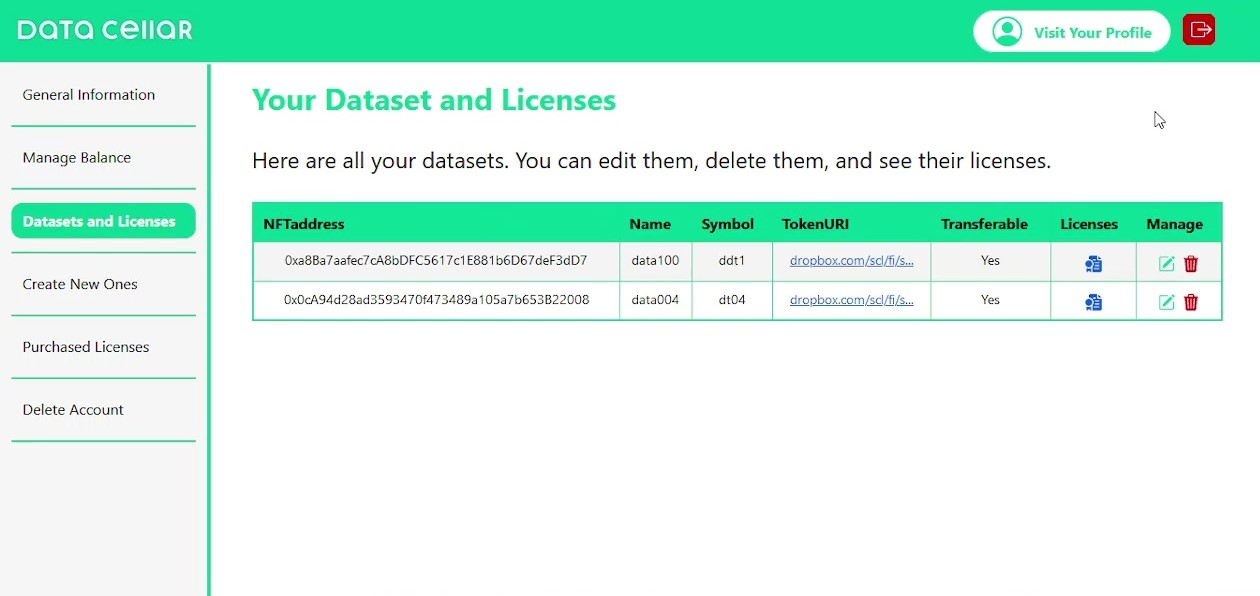
\includegraphics[width=0.8\textwidth]{Images/c6_8.jpg} 
    \caption{Page to view user's dataset and access their licenses.}
  \end{figure}

  \item \textbf{Create new Ones:} Here the user can create new datasets, i.e., add new datasets to the marketplace, or create new licenses related to an existing dataset 
  among its available ones. Datasets marked as transferable will be on the Home page of other users, allowing them to purchase their respective licenses.
  
  \begin{figure}[h]  
    \centering
    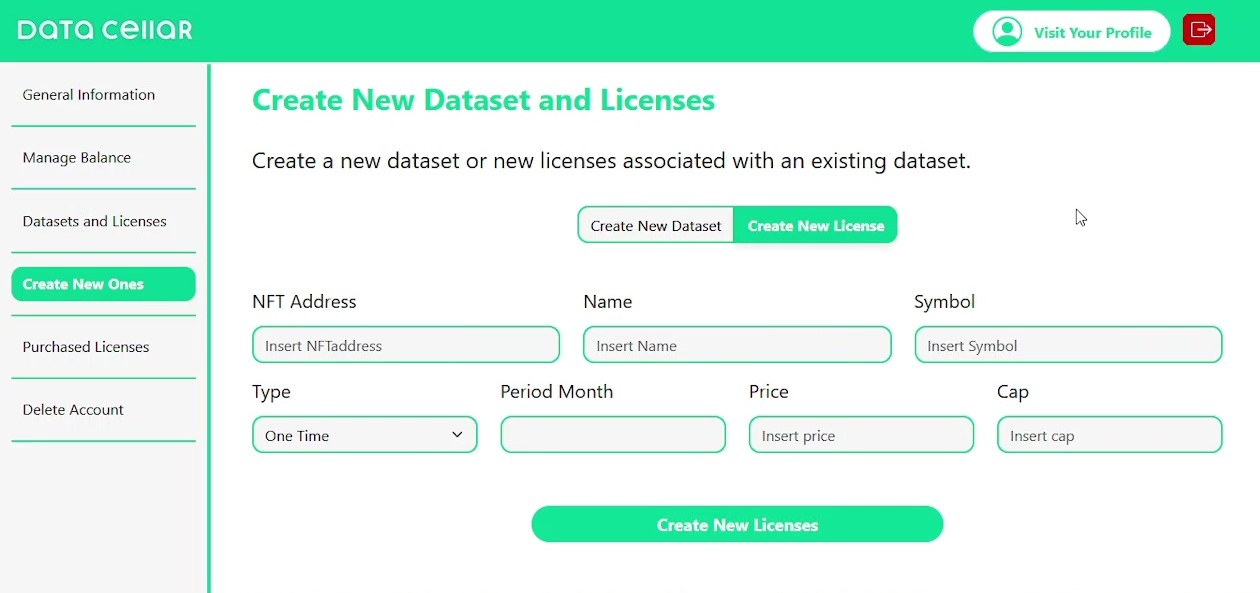
\includegraphics[width=0.8\textwidth]{Images/c6_9.jpg} 
    \caption{Page to create a new license or switch for new dataset. }
  \end{figure}
  
  \item \textbf{Purchased Licenses:} Shows the list of datasets for which the user has purchased at least one license. These licenses are visible by clicking on the 
  respective symbol leading to the dedicated page. Here the user can consume licenses, i.e., use them; periodic licenses can be used as many times as desired within the 
  validity period, while single-use licenses can be used a number of times equal to the amount of tokens available for it.
  
  \begin{figure}[h]  
    \centering
    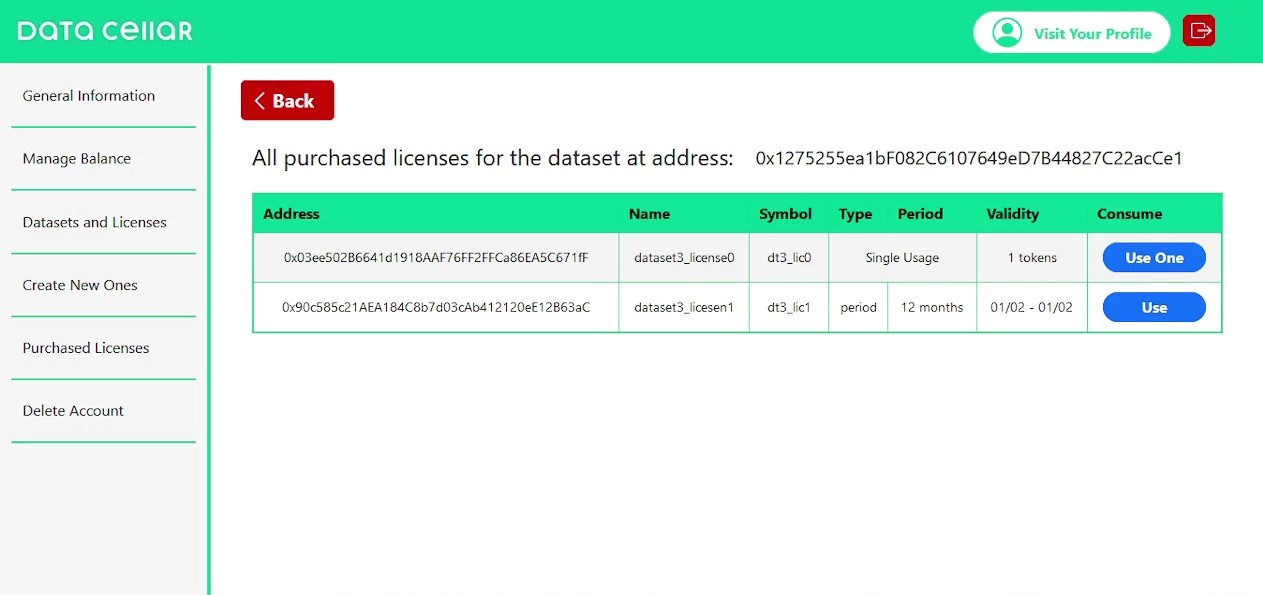
\includegraphics[width=0.8\textwidth]{Images/c6_10.jpg} 
    \caption{Page to view purchased licenses of specific dataset and use them.}
  \end{figure}
  
  \item \textbf{Delete Account:} This last page developed the latest smart contract function created for the \gls{ssi} management framework, which gives the user the ability to 
  delete their account, i.e., deregister. However, this function was not originally designed for this specific project, so it has limitations. In fact, by deleting an 
  account, the datasets, licenses and DataCellar tokens related to it and defined in the other smart contracts of the project are not deleted.

  \begin{figure}[h]  
    \centering
    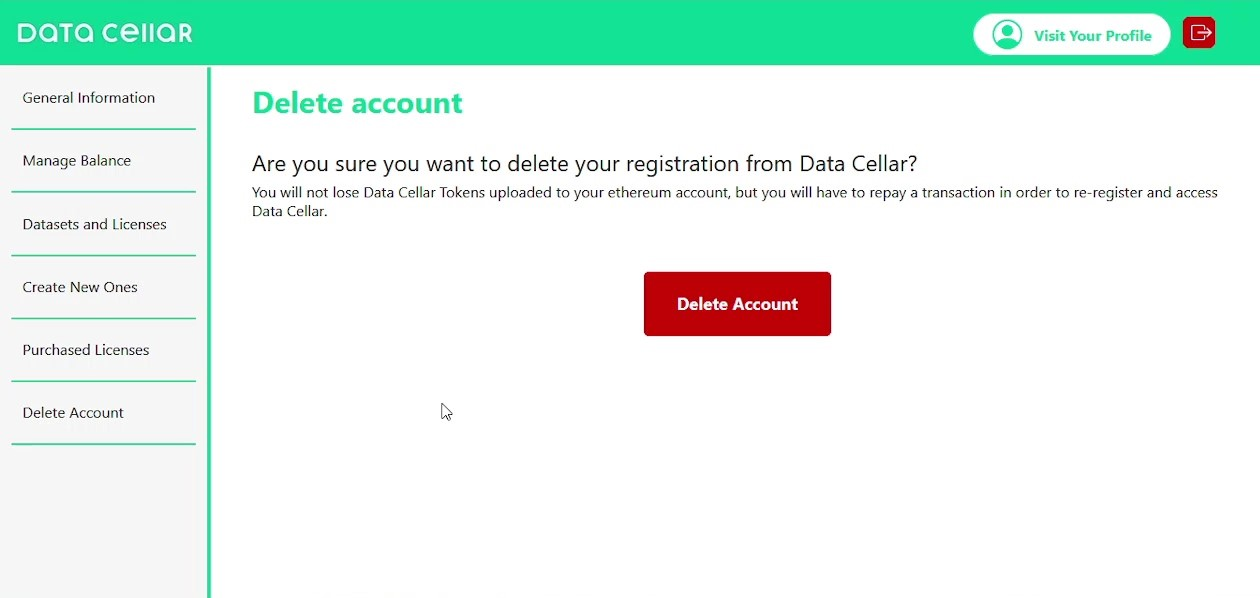
\includegraphics[width=0.8\textwidth]{Images/c6_11.jpg} 
    \caption{Page to delete user's account, performing de-registration.}
  \end{figure}

\end{itemize}

\chapter{Conclusions} \label{ch:conclusions}


%%%%%%%%%%%%%%%%%%%%%%%%%%%%%%%%%%%%%%%%%%%%%%%%
%%%%%%%%%%%%%%%%%%%%%%%%%%%%%%%%%%%%%%%%%%%%%%%%

\printbibliography

\end{document}